%% For double-blind review submission, w/o CCS and ACM Reference (max submission space)
\documentclass[acmsmall,review,anonymous]{acmart}\settopmatter{printfolios=true,printccs=false,printacmref=false}
%% For double-blind review submission, w/ CCS and ACM Reference
%\documentclass[acmsmall,review,anonymous]{acmart}\settopmatter{printfolios=true}
%% For single-blind review submission, w/o CCS and ACM Reference (max submission space)
%\documentclass[acmsmall,review]{acmart}\settopmatter{printfolios=true,printccs=false,printacmref=false}
%% For single-blind review submission, w/ CCS and ACM Reference
%\documentclass[acmsmall,review]{acmart}\settopmatter{printfolios=true}
%% For final camera-ready submission, w/ required CCS and ACM Reference
%\documentclass[acmsmall]{acmart}\settopmatter{}


%% Journal information
%% Supplied to authors by publisher for camera-ready submission;
%% use defaults for review submission.
\acmJournal{PACMPL}
\acmVolume{1}
\acmNumber{OOPSLA} % CONF = POPL or ICFP or OOPSLA
\acmArticle{1}
\acmYear{2018}
\acmMonth{1}
\acmDOI{} % \acmDOI{10.1145/nnnnnnn.nnnnnnn}
\startPage{1}

%% Copyright information
%% Supplied to authors (based on authors' rights management selection;
%% see authors.acm.org) by publisher for camera-ready submission;
%% use 'none' for review submission.
\setcopyright{none}
%\setcopyright{acmcopyright}
%\setcopyright{acmlicensed}
%\setcopyright{rightsretained}
%\copyrightyear{2018}           %% If different from \acmYear

%% Bibliography style
\bibliographystyle{ACM-Reference-Format}
%% Citation style
%% Note: author/year citations are required for papers published as an
%% issue of PACMPL.
\citestyle{acmauthoryear}   %% For author/year citations


%%%%%%%%%%%%%%%%%%%%%%%%%%%%%%%%%%%%%%%%%%%%%%%%%%%%%%%%%%%%%%%%%%%%%%
%% Note: Authors migrating a paper from PACMPL format to traditional
%% SIGPLAN proceedings format must update the '\documentclass' and
%% topmatter commands above; see 'acmart-sigplanproc-template.tex'.
%%%%%%%%%%%%%%%%%%%%%%%%%%%%%%%%%%%%%%%%%%%%%%%%%%%%%%%%%%%%%%%%%%%%%%


%\usepackage{cite}

\usepackage{amsmath,amssymb,amsfonts}
\usepackage[linesnumbered,ruled,vlined]{algorithm2e}

%\usepackage{graphicx}
\usepackage{textcomp}
\usepackage{xcolor}
\usepackage{caption}
\usepackage{subcaption}
\usepackage{multirow}
\usepackage{graphicx}
\usepackage{booktabs}
\usepackage{minted}
\usepackage{enumitem}
\usepackage{listings}
%\usepackage[breaklinks=true]{hyperref}
\usepackage{breakcites}
%\usepackage{algorithm} 
\usepackage{algorithmic}
\usepackage{tcolorbox}
\usepackage{multicol} 
\usepackage{subcaption}
\usepackage{ulem}
\usepackage{wrapfig}
\usepackage{amsmath}
\DeclareMathOperator*{\argmin}{arg\,min}
\DeclareMathOperator*{\argmax}{arg\,max}
\DeclareMathOperator*{\minimize}{minimize}

\begin{document}


%
\setlength\unitlength{1mm}
\newcommand{\twodots}{\mathinner {\ldotp \ldotp}}
% bb font symbols
\newcommand{\Rho}{\mathrm{P}}
\newcommand{\Tau}{\mathrm{T}}

\newfont{\bbb}{msbm10 scaled 700}
\newcommand{\CCC}{\mbox{\bbb C}}

\newfont{\bb}{msbm10 scaled 1100}
\newcommand{\CC}{\mbox{\bb C}}
\newcommand{\PP}{\mbox{\bb P}}
\newcommand{\RR}{\mbox{\bb R}}
\newcommand{\QQ}{\mbox{\bb Q}}
\newcommand{\ZZ}{\mbox{\bb Z}}
\newcommand{\FF}{\mbox{\bb F}}
\newcommand{\GG}{\mbox{\bb G}}
\newcommand{\EE}{\mbox{\bb E}}
\newcommand{\NN}{\mbox{\bb N}}
\newcommand{\KK}{\mbox{\bb K}}
\newcommand{\HH}{\mbox{\bb H}}
\newcommand{\SSS}{\mbox{\bb S}}
\newcommand{\UU}{\mbox{\bb U}}
\newcommand{\VV}{\mbox{\bb V}}


\newcommand{\yy}{\mathbbm{y}}
\newcommand{\xx}{\mathbbm{x}}
\newcommand{\zz}{\mathbbm{z}}
\newcommand{\sss}{\mathbbm{s}}
\newcommand{\rr}{\mathbbm{r}}
\newcommand{\pp}{\mathbbm{p}}
\newcommand{\qq}{\mathbbm{q}}
\newcommand{\ww}{\mathbbm{w}}
\newcommand{\hh}{\mathbbm{h}}
\newcommand{\vvv}{\mathbbm{v}}

% Vectors

\newcommand{\av}{{\bf a}}
\newcommand{\bv}{{\bf b}}
\newcommand{\cv}{{\bf c}}
\newcommand{\dv}{{\bf d}}
\newcommand{\ev}{{\bf e}}
\newcommand{\fv}{{\bf f}}
\newcommand{\gv}{{\bf g}}
\newcommand{\hv}{{\bf h}}
\newcommand{\iv}{{\bf i}}
\newcommand{\jv}{{\bf j}}
\newcommand{\kv}{{\bf k}}
\newcommand{\lv}{{\bf l}}
\newcommand{\mv}{{\bf m}}
\newcommand{\nv}{{\bf n}}
\newcommand{\ov}{{\bf o}}
\newcommand{\pv}{{\bf p}}
\newcommand{\qv}{{\bf q}}
\newcommand{\rv}{{\bf r}}
\newcommand{\sv}{{\bf s}}
\newcommand{\tv}{{\bf t}}
\newcommand{\uv}{{\bf u}}
\newcommand{\wv}{{\bf w}}
\newcommand{\vv}{{\bf v}}
\newcommand{\xv}{{\bf x}}
\newcommand{\yv}{{\bf y}}
\newcommand{\zv}{{\bf z}}
\newcommand{\zerov}{{\bf 0}}
\newcommand{\onev}{{\bf 1}}

% Matrices

\newcommand{\Am}{{\bf A}}
\newcommand{\Bm}{{\bf B}}
\newcommand{\Cm}{{\bf C}}
\newcommand{\Dm}{{\bf D}}
\newcommand{\Em}{{\bf E}}
\newcommand{\Fm}{{\bf F}}
\newcommand{\Gm}{{\bf G}}
\newcommand{\Hm}{{\bf H}}
\newcommand{\Id}{{\bf I}}
\newcommand{\Jm}{{\bf J}}
\newcommand{\Km}{{\bf K}}
\newcommand{\Lm}{{\bf L}}
\newcommand{\Mm}{{\bf M}}
\newcommand{\Nm}{{\bf N}}
\newcommand{\Om}{{\bf O}}
\newcommand{\Pm}{{\bf P}}
\newcommand{\Qm}{{\bf Q}}
\newcommand{\Rm}{{\bf R}}
\newcommand{\Sm}{{\bf S}}
\newcommand{\Tm}{{\bf T}}
\newcommand{\Um}{{\bf U}}
\newcommand{\Wm}{{\bf W}}
\newcommand{\Vm}{{\bf V}}
\newcommand{\Xm}{{\bf X}}
\newcommand{\Ym}{{\bf Y}}
\newcommand{\Zm}{{\bf Z}}

% Calligraphic

\newcommand{\Ac}{{\cal A}}
\newcommand{\Bc}{{\cal B}}
\newcommand{\Cc}{{\cal C}}
\newcommand{\Dc}{{\cal D}}
\newcommand{\Ec}{{\cal E}}
\newcommand{\Fc}{{\cal F}}
\newcommand{\Gc}{{\cal G}}
\newcommand{\Hc}{{\cal H}}
\newcommand{\Ic}{{\cal I}}
\newcommand{\Jc}{{\cal J}}
\newcommand{\Kc}{{\cal K}}
\newcommand{\Lc}{{\cal L}}
\newcommand{\Mc}{{\cal M}}
\newcommand{\Nc}{{\cal N}}
\newcommand{\nc}{{\cal n}}
\newcommand{\Oc}{{\cal O}}
\newcommand{\Pc}{{\cal P}}
\newcommand{\Qc}{{\cal Q}}
\newcommand{\Rc}{{\cal R}}
\newcommand{\Sc}{{\cal S}}
\newcommand{\Tc}{{\cal T}}
\newcommand{\Uc}{{\cal U}}
\newcommand{\Wc}{{\cal W}}
\newcommand{\Vc}{{\cal V}}
\newcommand{\Xc}{{\cal X}}
\newcommand{\Yc}{{\cal Y}}
\newcommand{\Zc}{{\cal Z}}

% Bold greek letters

\newcommand{\alphav}{\hbox{\boldmath$\alpha$}}
\newcommand{\betav}{\hbox{\boldmath$\beta$}}
\newcommand{\gammav}{\hbox{\boldmath$\gamma$}}
\newcommand{\deltav}{\hbox{\boldmath$\delta$}}
\newcommand{\etav}{\hbox{\boldmath$\eta$}}
\newcommand{\lambdav}{\hbox{\boldmath$\lambda$}}
\newcommand{\epsilonv}{\hbox{\boldmath$\epsilon$}}
\newcommand{\nuv}{\hbox{\boldmath$\nu$}}
\newcommand{\muv}{\hbox{\boldmath$\mu$}}
\newcommand{\zetav}{\hbox{\boldmath$\zeta$}}
\newcommand{\phiv}{\hbox{\boldmath$\phi$}}
\newcommand{\psiv}{\hbox{\boldmath$\psi$}}
\newcommand{\thetav}{\hbox{\boldmath$\theta$}}
\newcommand{\tauv}{\hbox{\boldmath$\tau$}}
\newcommand{\omegav}{\hbox{\boldmath$\omega$}}
\newcommand{\xiv}{\hbox{\boldmath$\xi$}}
\newcommand{\sigmav}{\hbox{\boldmath$\sigma$}}
\newcommand{\piv}{\hbox{\boldmath$\pi$}}
\newcommand{\rhov}{\hbox{\boldmath$\rho$}}
\newcommand{\upsilonv}{\hbox{\boldmath$\upsilon$}}

\newcommand{\Gammam}{\hbox{\boldmath$\Gamma$}}
\newcommand{\Lambdam}{\hbox{\boldmath$\Lambda$}}
\newcommand{\Deltam}{\hbox{\boldmath$\Delta$}}
\newcommand{\Sigmam}{\hbox{\boldmath$\Sigma$}}
\newcommand{\Phim}{\hbox{\boldmath$\Phi$}}
\newcommand{\Pim}{\hbox{\boldmath$\Pi$}}
\newcommand{\Psim}{\hbox{\boldmath$\Psi$}}
\newcommand{\Thetam}{\hbox{\boldmath$\Theta$}}
\newcommand{\Omegam}{\hbox{\boldmath$\Omega$}}
\newcommand{\Xim}{\hbox{\boldmath$\Xi$}}


% Sans Serif small case

\newcommand{\Gsf}{{\sf G}}

\newcommand{\asf}{{\sf a}}
\newcommand{\bsf}{{\sf b}}
\newcommand{\csf}{{\sf c}}
\newcommand{\dsf}{{\sf d}}
\newcommand{\esf}{{\sf e}}
\newcommand{\fsf}{{\sf f}}
\newcommand{\gsf}{{\sf g}}
\newcommand{\hsf}{{\sf h}}
\newcommand{\isf}{{\sf i}}
\newcommand{\jsf}{{\sf j}}
\newcommand{\ksf}{{\sf k}}
\newcommand{\lsf}{{\sf l}}
\newcommand{\msf}{{\sf m}}
\newcommand{\nsf}{{\sf n}}
\newcommand{\osf}{{\sf o}}
\newcommand{\psf}{{\sf p}}
\newcommand{\qsf}{{\sf q}}
\newcommand{\rsf}{{\sf r}}
\newcommand{\ssf}{{\sf s}}
\newcommand{\tsf}{{\sf t}}
\newcommand{\usf}{{\sf u}}
\newcommand{\wsf}{{\sf w}}
\newcommand{\vsf}{{\sf v}}
\newcommand{\xsf}{{\sf x}}
\newcommand{\ysf}{{\sf y}}
\newcommand{\zsf}{{\sf z}}


% mixed symbols

\newcommand{\sinc}{{\hbox{sinc}}}
\newcommand{\diag}{{\hbox{diag}}}
\renewcommand{\det}{{\hbox{det}}}
\newcommand{\trace}{{\hbox{tr}}}
\newcommand{\sign}{{\hbox{sign}}}
\renewcommand{\arg}{{\hbox{arg}}}
\newcommand{\var}{{\hbox{var}}}
\newcommand{\cov}{{\hbox{cov}}}
\newcommand{\Ei}{{\rm E}_{\rm i}}
\renewcommand{\Re}{{\rm Re}}
\renewcommand{\Im}{{\rm Im}}
\newcommand{\eqdef}{\stackrel{\Delta}{=}}
\newcommand{\defines}{{\,\,\stackrel{\scriptscriptstyle \bigtriangleup}{=}\,\,}}
\newcommand{\<}{\left\langle}
\renewcommand{\>}{\right\rangle}
\newcommand{\herm}{{\sf H}}
\newcommand{\trasp}{{\sf T}}
\newcommand{\transp}{{\sf T}}
\renewcommand{\vec}{{\rm vec}}
\newcommand{\Psf}{{\sf P}}
\newcommand{\SINR}{{\sf SINR}}
\newcommand{\SNR}{{\sf SNR}}
\newcommand{\MMSE}{{\sf MMSE}}
\newcommand{\REF}{{\RED [REF]}}

% Markov chain
\usepackage{stmaryrd} % for \mkv 
\newcommand{\mkv}{-\!\!\!\!\minuso\!\!\!\!-}

% Colors

\newcommand{\RED}{\color[rgb]{1.00,0.10,0.10}}
\newcommand{\BLUE}{\color[rgb]{0,0,0.90}}
\newcommand{\GREEN}{\color[rgb]{0,0.80,0.20}}

%%%%%%%%%%%%%%%%%%%%%%%%%%%%%%%%%%%%%%%%%%
\usepackage{hyperref}
\hypersetup{
    bookmarks=true,         % show bookmarks bar?
    unicode=false,          % non-Latin characters in AcrobatÕs bookmarks
    pdftoolbar=true,        % show AcrobatÕs toolbar?
    pdfmenubar=true,        % show AcrobatÕs menu?
    pdffitwindow=false,     % window fit to page when opened
    pdfstartview={FitH},    % fits the width of the page to the window
%    pdftitle={My title},    % title
%    pdfauthor={Author},     % author
%    pdfsubject={Subject},   % subject of the document
%    pdfcreator={Creator},   % creator of the document
%    pdfproducer={Producer}, % producer of the document
%    pdfkeywords={keyword1} {key2} {key3}, % list of keywords
    pdfnewwindow=true,      % links in new window
    colorlinks=true,       % false: boxed links; true: colored links
    linkcolor=red,          % color of internal links (change box color with linkbordercolor)
    citecolor=green,        % color of links to bibliography
    filecolor=blue,      % color of file links
    urlcolor=blue           % color of external links
}
%%%%%%%%%%%%%%%%%%%%%%%%%%%%%%%%%%%%%%%%%%%


%% Title information
\title{CodeImprove: Program Adaptation for Deep Code Models}         %% [Short Title] is optional;
                                        %% when present, will be used in
                                        %% header instead of Full Title.
%\titlenote{with title note}             %% \titlenote is optional;
                                        %% can be repeated if necessary;
                                        %% contents suppressed with 'anonymous'
%\subtitle{Subtitle}                     %% \subtitle is optional
%\subtitlenote{with subtitle note}       %% \subtitlenote is optional;
                                        %% can be repeated if necessary;
                                        %% contents suppressed with 'anonymous'


%% Author information
%% Contents and number of authors suppressed with 'anonymous'.
%% Each author should be introduced by \author, followed by
%% \authornote (optional), \orcid (optional), \affiliation, and
%% \email.
%% An author may have multiple affiliations and/or emails; repeat the
%% appropriate command.
%% Many elements are not rendered, but should be provided for metadata
%% extraction tools.

%% Author with single affiliation.
\author{First1 Last1}
\authornote{with author1 note}          %% \authornote is optional;
                                        %% can be repeated if necessary
\orcid{nnnn-nnnn-nnnn-nnnn}             %% \orcid is optional
\affiliation{
  \position{Position1}
  \department{Department1}              %% \department is recommended
  \institution{Institution1}            %% \institution is required
  \streetaddress{Street1 Address1}
  \city{City1}
  \state{State1}
  \postcode{Post-Code1}
  \country{Country1}                    %% \country is recommended
}
\email{first1.last1@inst1.edu}          %% \email is recommended

%% Author with two affiliations and emails.
\author{First2 Last2}
\authornote{with author2 note}          %% \authornote is optional;
                                        %% can be repeated if necessary
\orcid{nnnn-nnnn-nnnn-nnnn}             %% \orcid is optional
\affiliation{
  \position{Position2a}
  \department{Department2a}             %% \department is recommended
  \institution{Institution2a}           %% \institution is required
  \streetaddress{Street2a Address2a}
  \city{City2a}
  \state{State2a}
  \postcode{Post-Code2a}
  \country{Country2a}                   %% \country is recommended
}
\email{first2.last2@inst2a.com}         %% \email is recommended
\affiliation{
  \position{Position2b}
  \department{Department2b}             %% \department is recommended
  \institution{Institution2b}           %% \institution is required
  \streetaddress{Street3b Address2b}
  \city{City2b}
  \state{State2b}
  \postcode{Post-Code2b}
  \country{Country2b}                   %% \country is recommended
}
\email{first2.last2@inst2b.org}         %% \email is recommended


%% Abstract
%% Note: \begin{abstract}...\end{abstract} environment must come
%% before \maketitle command
\begin{abstract}
\begin{abstract}  
Test time scaling is currently one of the most active research areas that shows promise after training time scaling has reached its limits.
Deep-thinking (DT) models are a class of recurrent models that can perform easy-to-hard generalization by assigning more compute to harder test samples.
However, due to their inability to determine the complexity of a test sample, DT models have to use a large amount of computation for both easy and hard test samples.
Excessive test time computation is wasteful and can cause the ``overthinking'' problem where more test time computation leads to worse results.
In this paper, we introduce a test time training method for determining the optimal amount of computation needed for each sample during test time.
We also propose Conv-LiGRU, a novel recurrent architecture for efficient and robust visual reasoning. 
Extensive experiments demonstrate that Conv-LiGRU is more stable than DT, effectively mitigates the ``overthinking'' phenomenon, and achieves superior accuracy.
\end{abstract}  
\end{abstract}


%% 2012 ACM Computing Classification System (CSS) concepts
%% Generate at 'http://dl.acm.org/ccs/ccs.cfm'.
\begin{CCSXML}
<ccs2012>
<concept>
<concept_id>10011007.10011006.10011008</concept_id>
<concept_desc>Software and its engineering~General programming languages</concept_desc>
<concept_significance>500</concept_significance>
</concept>
<concept>
<concept_id>10003456.10003457.10003521.10003525</concept_id>
<concept_desc>Social and professional topics~History of programming languages</concept_desc>
<concept_significance>300</concept_significance>
</concept>
</ccs2012>
\end{CCSXML}

\ccsdesc[500]{Software and its engineering~General programming languages}
\ccsdesc[300]{Social and professional topics~History of programming languages}
%% End of generated code


%% Keywords
%% comma separated list
\keywords{Input validation, Program adaptation, Program transformation }  %% \keywords are mandatory in final camera-ready submission


%% \maketitle
%% Note: \maketitle command must come after title commands, author
%% commands, abstract environment, Computing Classification System
%% environment and commands, and keywords command.
\maketitle

\section{Introduction}
\label{sec:introduction}
The business processes of organizations are experiencing ever-increasing complexity due to the large amount of data, high number of users, and high-tech devices involved \cite{martin2021pmopportunitieschallenges, beerepoot2023biggestbpmproblems}. This complexity may cause business processes to deviate from normal control flow due to unforeseen and disruptive anomalies \cite{adams2023proceddsriftdetection}. These control-flow anomalies manifest as unknown, skipped, and wrongly-ordered activities in the traces of event logs monitored from the execution of business processes \cite{ko2023adsystematicreview}. For the sake of clarity, let us consider an illustrative example of such anomalies. Figure \ref{FP_ANOMALIES} shows a so-called event log footprint, which captures the control flow relations of four activities of a hypothetical event log. In particular, this footprint captures the control-flow relations between activities \texttt{a}, \texttt{b}, \texttt{c} and \texttt{d}. These are the causal ($\rightarrow$) relation, concurrent ($\parallel$) relation, and other ($\#$) relations such as exclusivity or non-local dependency \cite{aalst2022pmhandbook}. In addition, on the right are six traces, of which five exhibit skipped, wrongly-ordered and unknown control-flow anomalies. For example, $\langle$\texttt{a b d}$\rangle$ has a skipped activity, which is \texttt{c}. Because of this skipped activity, the control-flow relation \texttt{b}$\,\#\,$\texttt{d} is violated, since \texttt{d} directly follows \texttt{b} in the anomalous trace.
\begin{figure}[!t]
\centering
\includegraphics[width=0.9\columnwidth]{images/FP_ANOMALIES.png}
\caption{An example event log footprint with six traces, of which five exhibit control-flow anomalies.}
\label{FP_ANOMALIES}
\end{figure}

\subsection{Control-flow anomaly detection}
Control-flow anomaly detection techniques aim to characterize the normal control flow from event logs and verify whether these deviations occur in new event logs \cite{ko2023adsystematicreview}. To develop control-flow anomaly detection techniques, \revision{process mining} has seen widespread adoption owing to process discovery and \revision{conformance checking}. On the one hand, process discovery is a set of algorithms that encode control-flow relations as a set of model elements and constraints according to a given modeling formalism \cite{aalst2022pmhandbook}; hereafter, we refer to the Petri net, a widespread modeling formalism. On the other hand, \revision{conformance checking} is an explainable set of algorithms that allows linking any deviations with the reference Petri net and providing the fitness measure, namely a measure of how much the Petri net fits the new event log \cite{aalst2022pmhandbook}. Many control-flow anomaly detection techniques based on \revision{conformance checking} (hereafter, \revision{conformance checking}-based techniques) use the fitness measure to determine whether an event log is anomalous \cite{bezerra2009pmad, bezerra2013adlogspais, myers2018icsadpm, pecchia2020applicationfailuresanalysispm}. 

The scientific literature also includes many \revision{conformance checking}-independent techniques for control-flow anomaly detection that combine specific types of trace encodings with machine/deep learning \cite{ko2023adsystematicreview, tavares2023pmtraceencoding}. Whereas these techniques are very effective, their explainability is challenging due to both the type of trace encoding employed and the machine/deep learning model used \cite{rawal2022trustworthyaiadvances,li2023explainablead}. Hence, in the following, we focus on the shortcomings of \revision{conformance checking}-based techniques to investigate whether it is possible to support the development of competitive control-flow anomaly detection techniques while maintaining the explainable nature of \revision{conformance checking}.
\begin{figure}[!t]
\centering
\includegraphics[width=\columnwidth]{images/HIGH_LEVEL_VIEW.png}
\caption{A high-level view of the proposed framework for combining \revision{process mining}-based feature extraction with dimensionality reduction for control-flow anomaly detection.}
\label{HIGH_LEVEL_VIEW}
\end{figure}

\subsection{Shortcomings of \revision{conformance checking}-based techniques}
Unfortunately, the detection effectiveness of \revision{conformance checking}-based techniques is affected by noisy data and low-quality Petri nets, which may be due to human errors in the modeling process or representational bias of process discovery algorithms \cite{bezerra2013adlogspais, pecchia2020applicationfailuresanalysispm, aalst2016pm}. Specifically, on the one hand, noisy data may introduce infrequent and deceptive control-flow relations that may result in inconsistent fitness measures, whereas, on the other hand, checking event logs against a low-quality Petri net could lead to an unreliable distribution of fitness measures. Nonetheless, such Petri nets can still be used as references to obtain insightful information for \revision{process mining}-based feature extraction, supporting the development of competitive and explainable \revision{conformance checking}-based techniques for control-flow anomaly detection despite the problems above. For example, a few works outline that token-based \revision{conformance checking} can be used for \revision{process mining}-based feature extraction to build tabular data and develop effective \revision{conformance checking}-based techniques for control-flow anomaly detection \cite{singh2022lapmsh, debenedictis2023dtadiiot}. However, to the best of our knowledge, the scientific literature lacks a structured proposal for \revision{process mining}-based feature extraction using the state-of-the-art \revision{conformance checking} variant, namely alignment-based \revision{conformance checking}.

\subsection{Contributions}
We propose a novel \revision{process mining}-based feature extraction approach with alignment-based \revision{conformance checking}. This variant aligns the deviating control flow with a reference Petri net; the resulting alignment can be inspected to extract additional statistics such as the number of times a given activity caused mismatches \cite{aalst2022pmhandbook}. We integrate this approach into a flexible and explainable framework for developing techniques for control-flow anomaly detection. The framework combines \revision{process mining}-based feature extraction and dimensionality reduction to handle high-dimensional feature sets, achieve detection effectiveness, and support explainability. Notably, in addition to our proposed \revision{process mining}-based feature extraction approach, the framework allows employing other approaches, enabling a fair comparison of multiple \revision{conformance checking}-based and \revision{conformance checking}-independent techniques for control-flow anomaly detection. Figure \ref{HIGH_LEVEL_VIEW} shows a high-level view of the framework. Business processes are monitored, and event logs obtained from the database of information systems. Subsequently, \revision{process mining}-based feature extraction is applied to these event logs and tabular data input to dimensionality reduction to identify control-flow anomalies. We apply several \revision{conformance checking}-based and \revision{conformance checking}-independent framework techniques to publicly available datasets, simulated data of a case study from railways, and real-world data of a case study from healthcare. We show that the framework techniques implementing our approach outperform the baseline \revision{conformance checking}-based techniques while maintaining the explainable nature of \revision{conformance checking}.

In summary, the contributions of this paper are as follows.
\begin{itemize}
    \item{
        A novel \revision{process mining}-based feature extraction approach to support the development of competitive and explainable \revision{conformance checking}-based techniques for control-flow anomaly detection.
    }
    \item{
        A flexible and explainable framework for developing techniques for control-flow anomaly detection using \revision{process mining}-based feature extraction and dimensionality reduction.
    }
    \item{
        Application to synthetic and real-world datasets of several \revision{conformance checking}-based and \revision{conformance checking}-independent framework techniques, evaluating their detection effectiveness and explainability.
    }
\end{itemize}

The rest of the paper is organized as follows.
\begin{itemize}
    \item Section \ref{sec:related_work} reviews the existing techniques for control-flow anomaly detection, categorizing them into \revision{conformance checking}-based and \revision{conformance checking}-independent techniques.
    \item Section \ref{sec:abccfe} provides the preliminaries of \revision{process mining} to establish the notation used throughout the paper, and delves into the details of the proposed \revision{process mining}-based feature extraction approach with alignment-based \revision{conformance checking}.
    \item Section \ref{sec:framework} describes the framework for developing \revision{conformance checking}-based and \revision{conformance checking}-independent techniques for control-flow anomaly detection that combine \revision{process mining}-based feature extraction and dimensionality reduction.
    \item Section \ref{sec:evaluation} presents the experiments conducted with multiple framework and baseline techniques using data from publicly available datasets and case studies.
    \item Section \ref{sec:conclusions} draws the conclusions and presents future work.
\end{itemize}
\section{Background}\label{sec:backgrnd}

\subsection{Cold Start Latency and Mitigation Techniques}

Traditional FaaS platforms mitigate cold starts through snapshotting, lightweight virtualization, and warm-state management. Snapshot-based methods like \textbf{REAP} and \textbf{Catalyzer} reduce initialization time by preloading or restoring container states but require significant memory and I/O resources, limiting scalability~\cite{dong_catalyzer_2020, ustiugov_benchmarking_2021}. Lightweight virtualization solutions, such as \textbf{Firecracker} microVMs, achieve fast startup times with strong isolation but depend on robust infrastructure, making them less adaptable to fluctuating workloads~\cite{agache_firecracker_2020}. Warm-state management techniques like \textbf{Faa\$T}~\cite{romero_faa_2021} and \textbf{Kraken}~\cite{vivek_kraken_2021} keep frequently invoked containers ready, balancing readiness and cost efficiency under predictable workloads but incurring overhead when demand is erratic~\cite{romero_faa_2021, vivek_kraken_2021}. While these methods perform well in resource-rich cloud environments, their resource intensity challenges applicability in edge settings.

\subsubsection{Edge FaaS Perspective}

In edge environments, cold start mitigation emphasizes lightweight designs, resource sharing, and hybrid task distribution. Lightweight execution environments like unikernels~\cite{edward_sock_2018} and \textbf{Firecracker}~\cite{agache_firecracker_2020}, as used by \textbf{TinyFaaS}~\cite{pfandzelter_tinyfaas_2020}, minimize resource usage and initialization delays but require careful orchestration to avoid resource contention. Function co-location, demonstrated by \textbf{Photons}~\cite{v_dukic_photons_2020}, reduces redundant initializations by sharing runtime resources among related functions, though this complicates isolation in multi-tenant setups~\cite{v_dukic_photons_2020}. Hybrid offloading frameworks like \textbf{GeoFaaS}~\cite{malekabbasi_geofaas_2024} balance edge-cloud workloads by offloading latency-tolerant tasks to the cloud and reserving edge resources for real-time operations, requiring reliable connectivity and efficient task management. These edge-specific strategies address cold starts effectively but introduce challenges in scalability and orchestration.

\subsection{Predictive Scaling and Caching Techniques}

Efficient resource allocation is vital for maintaining low latency and high availability in serverless platforms. Predictive scaling and caching techniques dynamically provision resources and reduce cold start latency by leveraging workload prediction and state retention.
Traditional FaaS platforms use predictive scaling and caching to optimize resources, employing techniques (OFC, FaasCache) to reduce cold starts. However, these methods rely on centralized orchestration and workload predictability, limiting their effectiveness in dynamic, resource-constrained edge environments.



\subsubsection{Edge FaaS Perspective}

Edge FaaS platforms adapt predictive scaling and caching techniques to constrain resources and heterogeneous environments. \textbf{EDGE-Cache}~\cite{kim_delay-aware_2022} uses traffic profiling to selectively retain high-priority functions, reducing memory overhead while maintaining readiness for frequent requests. Hybrid frameworks like \textbf{GeoFaaS}~\cite{malekabbasi_geofaas_2024} implement distributed caching to balance resources between edge and cloud nodes, enabling low-latency processing for critical tasks while offloading less critical workloads. Machine learning methods, such as clustering-based workload predictors~\cite{gao_machine_2020} and GRU-based models~\cite{guo_applying_2018}, enhance resource provisioning in edge systems by efficiently forecasting workload spikes. These innovations effectively address cold start challenges in edge environments, though their dependency on accurate predictions and robust orchestration poses scalability challenges.

\subsection{Decentralized Orchestration, Function Placement, and Scheduling}

Efficient orchestration in serverless platforms involves workload distribution, resource optimization, and performance assurance. While traditional FaaS platforms rely on centralized control, edge environments require decentralized and adaptive strategies to address unique challenges such as resource constraints and heterogeneous hardware.



\subsubsection{Edge FaaS Perspective}

Edge FaaS platforms adopt decentralized and adaptive orchestration frameworks to meet the demands of resource-constrained environments. Systems like \textbf{Wukong} distribute scheduling across edge nodes, enhancing data locality and scalability while reducing network latency. Lightweight frameworks such as \textbf{OpenWhisk Lite}~\cite{kravchenko_kpavelopenwhisk-light_2024} optimize resource allocation by decentralizing scheduling policies, minimizing cold starts and latency in edge setups~\cite{benjamin_wukong_2020}. Hybrid solutions like \textbf{OpenFaaS}~\cite{noauthor_openfaasfaas_2024} and \textbf{EdgeMatrix}~\cite{shen_edgematrix_2023} combine edge-cloud orchestration to balance resource utilization, retaining latency-sensitive functions at the edge while offloading non-critical workloads to the cloud. While these approaches improve flexibility, they face challenges in maintaining coordination and ensuring consistent performance across distributed nodes.



% Consider a lasso optimization procedure with potentially distinct regularization penalties:
% \begin{align}
%     \hat{\beta} = \arg\min_{\beta}\{\|y-X\beta\|^2_2+\sum_{i=1}^{N}\lambda_i|\beta_i|\}.
% \end{align}
\subsection{Supervised Data-Driven Learning}\label{subsec:supervised}
We consider a generic data-driven supervised learning procedure. Given a dataset \( \mathcal{D} \) consisting of \( n \) data points \( (x_i, y_i) \in \mathcal{X} \times \mathcal{Y} \) drawn from an underlying distribution \( p(\cdot|\theta) \), our goal is to estimate parameters \( \theta \in \Theta \) through a learning procedure, defined as \( f: (\mathcal{X} \times \mathcal{Y})^n \rightarrow \Theta \) 
that minimizes the predictive error on observed data. 
Specifically, the learning objective is defined as follows:
\begin{align}
\hat{\theta}_f := f(\mathcal{D}) = \arg\min_{\theta} \mathcal{L}(\theta, \mathcal{D}),
\end{align}
where \( \mathcal{L}(\cdot,\mathcal{D}) := \sum_{i=1}^{n} \mathcal{L}(\cdot, (x_i, y_i))\), and $\mathcal{L}$ is a loss function quantifying the error between predictions and true outcomes. 
Here, $\hat{\theta}_f$ is the parameter that best explains the observed data pairs \( (x_i, y_i) \) according to the chosen loss function \( \mathcal{L} (\cdot) \).

\paragraph{Feature Selection.}
Feature selection aims to improve model \( f \)'s predictive performance while minimizing redundancy. 
%Formally, given data \( X \), response \( y \), feature set \( \mathcal{F} \), loss function \( \mathcal{L}(\cdot) \), and a feature limit \( k \), the objective is:
% \begin{align}
% \mathcal{S}^* = \arg \min_{\mathcal{S} \subseteq \mathcal{F}, |\mathcal{S}| \leq k} \mathcal{L}(y, f(X_\mathcal{S})) + \lambda R(\mathcal{S}),
% \end{align}
% where \( X_\mathcal{S} \) is the submatrix of \( X \) for selected features \( \mathcal{S} \), \( \lambda \) is a regularization parameter, and \( R(\mathcal{S}) \) penalizes feature redundancy.
 State-of-the-art techniques fall into four categories: (i) filter methods, which rank features based on statistical properties like Fisher score \citep{duda2001pattern,song2012feature}; (ii) wrapper methods, which evaluate model performance on different feature subsets \citep{kohavi1997wrappers}; (iii) embedded methods, which integrate feature selection into the learning process using techniques like regularization \citep{tibshirani1996LASSO,lemhadri2021lassonet}; and (iv) hybrid methods, which combine elements of (i)-(iii) \citep{SINGH2021104396,li2022micq}. This paper focuses on embedded methods via Lasso, benchmarking against approaches from (i)-(iii).

\subsection{Language Modeling}
% The objective of language modeling is to learn a probability distribution \( p_{LM}(x) \) over sequences of text \( x = (X_1, \ldots, X_{|x|}) \), such that \( p_{LM}(x) \approx p_{text}(x) \), where \( p_{text}(x) \) represents the true distribution of natural language. This process involves estimating the likelihood of token sequences across variable lengths and diverse linguistic structures.
% Modern large language models (LLMs) are trained on vast datasets spanning encyclopedias, news, social media, books, and scientific papers \cite{gao2020pile}. This broad training enables them to generalize across domains, learn contextual knowledge, and perform zero-shot learning—tackling new tasks using only task descriptions without fine-tuning \cite{brown2020gpt3}.
Language modeling aims to approximate the true distribution of natural language \( p_{\text{text}}(x) \) by learning \( p_{\text{LM}}(x) \), a probability distribution over text sequences \( x = (X_1, \ldots, X_{|x|}) \). Modern large language models, trained on diverse datasets \citep{gao2020pile}, exhibit strong generalization across domains, acquire contextual knowledge, and perform zero-shot learning—solving new tasks using only task descriptions—or few-shot learning by leveraging a small number of demonstrations \citep{brown2020gpt3}.
\paragraph{Retrieval-Augmented Generation (RAG).} Retrieval-Augmented Generation (RAG) enhances the performance of generative language models by  integrating a domain-specific information retrieval process  \citep{lewis2020retrieval}. The RAG framework comprises two main components: \textit{retrieval}, which extracts relevant information from external knowledge sources, and \textit{generation}, where an LLM generates context-aware responses using the prompt combined with the retrieved context. Documents are indexed through various databases, such as relational, graph, or vector databases \citep{khattab2020colbert, douze2024faiss, peng2024graphretrievalaugmentedgenerationsurvey}, enabling efficient organization and retrieval via algorithms like semantic similarity search to match the prompt with relevant documents in the knowledge base. RAG has gained much traction recently due to its demonstrated ability to reduce incidence of hallucinations and boost LLMs' reliability as well as performance \citep{huang2023hallucination, zhang2023merging}. 
 
% image source: https://medium.com/@bindurani_22/retrieval-augmented-generation-815c1ae438d8
\begin{figure}
    \centering
\includegraphics[width=1.03\linewidth]{fig/fig1.pdf}
\vspace{-0.6cm}
\scriptsize 
    \caption{Retrieval Augmented Generation (RAG) based $\ell_1$-norm weights (penalty factors) for Lasso. Only feature names---no training data--- are included in LLM prompt.} 
    \label{fig:rag}
\end{figure}
% However, for the RAG model to be effective given the input token constraints of the LLM model used, we need to effectively process the retrieval documents through a procedure known as \textit{chunking}.

\subsection{Task-Specific Data-Driven Learning}
LLM-Lasso aims to bridge the gap between data-driven supervised learning and the predictive capabilities of LLMs trained on rich metadata. This fusion not only enhances traditional data-driven methods by incorporating key task-relevant contextual information often overlooked by such models, but can also be especially valuable in low-data regimes, where the learning algorithm $f:\mathcal{D}\rightarrow\Theta$ (seen as a map from datasets $\mathcal{D}$ to the space of decisions $\Theta$) is susceptible to overfitting.

The task-specific data-driven learning model $\tilde{f}:\mathcal{D}\times\mathcal{D}_\text{meta}\rightarrow\Theta$ can be described as a metadata-augmented version of $f$, where a link function $h(\cdot)$ integrates metadata (i.e. $\mathcal{D}_\text{meta}$) to refine the original learning process. This can be expressed as:
\[
\tilde{f}(\mathcal{D}, \mathcal{D}_\text{meta}) := \mathcal{T}(f(\mathcal{D}),  h(\mathcal{D}_{\text{meta}})),
\]
where the functional $\mathcal{T}$ takes the original learning algorithm $f(\mathcal{D})$ and transforms it into a task-specific learning algorithm $\tilde{f}(\mathcal{D}, \mathcal{D}_\text{meta})$ by incorporating the metadata $\mathcal{D}_\text{meta}$. 
% In particular, the link function $h(\mathcal{D}_{\text{meta}})$ provides a structured mechanism summarizing the contextual knowledge.

There are multiple approaches to formulate $\mathcal{T}$ and $h$.
%to ``inform" the data-driven model $f$ of %meta knowledge. 
For instance, LMPriors \citep{choi2022lmpriorspretrainedlanguagemodels} designed $h$ and $\mathcal{T}$ such that $h(\mathcal{D}_{\text{meta}})$ first specifies which features to retain (based on a probabilistic prior framework), and then $\mathcal{T}$ keeps the selected features and removes all the others from the original learning objective of $f$. 
Note that this approach inherently is restricted as it selects important features solely based on $\mathcal{D}_\text{meta}$ without seeing $\mathcal{D}$.

In contrast, we directly embed task-specific knowledge into the optimization landscape through regularization by introducing a structured inductive bias. This bias guides the learning process toward solutions that are consistent with metadata-informed insights, without relying on explicit probabilistic modeling. Abstractly, this can be expressed as:
\begin{align}
    \!\!\!\!\!\hat{\theta}_{\tilde{f}} := \tilde{f}(\mathcal{D},\mathcal{D}
    _\text{meta})= \arg\min_{\theta} \mathcal{L}(\theta, \mathcal{D}) + \lambda R(\theta, \mathcal{D}_{\text{meta}}),
\end{align}
where \( \lambda \) is a regularization parameter, \( R(\cdot) \) is a regularizer, and $\theta$ is the prediction parameter.
%We explain our framework with more details in the following section.


% Our research diverges from both aforementioned approaches by positioning the LLM not as a standalone feature selector but as an enhancement to data-driven models through an embedded feature selection method, L-LASSO. L-LASSO incorporates domain expertise—auxiliary natural language metadata about the task—via the LLM-informed LASSO penalty, which is then used in statistical models to enhance predictive performance. This method integrates the rich, context-sensitive insights of LLMs with the rigor and transparency of statistical modeling, bridging the gap between data-driven and knowledge-driven feature selection approaches. To approach this task, we need to tackle two key components: (i). train an LLM that is expert in the task-specific knowledge; (ii). inform data-driven feature selector LASSO with LLM knowledge.

% In practice, this involves combining techniques like prompt engineering and data engineering to develop an effective framework for integrating metadata into existing data-driven models. We will go through this in detail in Section \ref{mthd} and \ref{experiment}.


\section{The \search\ Search Algorithm}
\label{sec:search}

%In traditional ML, structure changes and step (operator) changes are performed before model training, \ie, fixed to the training process, and weights are updated with SGD, because weights are continous, differentiable values, and there are significantly more weights than structure and operator changes. In workflow autotuning, all three types of cogs can be chosen with a unified search-based approach, because all of them are non-differentiable configurations and the number of cogs in different types are all small.
%Thus, \sysname\ only needs to navigate the search space of combination of cogs as the search space to produce its workflow optimization results.

%We propose, \textit{\textbf{\search}}, an adaptive hierarchical search algorithm that autotunes gen-AI workflows based on observed end-to-end workflow results. In each search iteration, \search\ selects a combination of cogs to apply to the workflow and executes the resulting workflow with user-provided training inputs. \search\ evaluates the final generation quality using the user-specified evaluator and measures the execution time and cost for each training input. These results are aggregated and serve as BO observations and pruning criteria.
%the optimizer can condition on and propose better configurations in later trials. The optimizer will also be informed about the violation of any user-specified metric thresholds. More details of this mechanism can be found in Appendix ~\ref{appdx:TPE}.

With our insights in Section~\ref{sec:theory}, we believe that search methods based on Bayesian Optimizer (BO) can work for all types of cogs in gen-AI workflow autotuning because of BO's efficiency in searching discrete search space.
A key challenge in designing a BO-based search is the limited search budgets that need to be used to search a high-dimensional cog space. 
For example, for 4 cogs each with 4 options and a workflow of 3 LLM steps, the search space is $4^{12}$. Suppose each search uses GPT-4o and has 1000 output tokens, the entire space needs around \$168K to go through. A user search budget of \$100 can cover only 0.06\% of the search space. A traditional BO approach cannot find good results with such small budgets.
%The entire search space grows exponentially with the number of cogs and the number of steps in a workflow. Moreover, different cogs and different combinations of cogs can have varying impacts on different workflows. 
%Without prior knowledge, it is difficult to determine the amount of budget to give to each cog.

To confront this challenge, we propose \textit{\textbf{\search}}, an adaptive hierarchical search algorithm that efficiently assigns search budget across cogs based on budget size and observed workflow evaluation results, as defined in Algorithms~\ref{alg:main} and \ref{alg:outer} and described below.
%autotunes gen-AI workflows based on observed end-to-end workflow results.
%\search\ includes a search layer partitioning method, a search budget initial assignment method, an evaluation-guided budget re-allocation mechanism, and a convergence-based early-exiting strategy. We discuss them in details below.

%\zijian{\search\ allows users to specify the optimization budget allowed in terms of the maximum number of search iterations. Based on the relationship between the complexity of the search space and the available budget, we will separate all tunable parameters into different layers each optimized by independent Bayesian optimization routines. Then we will decide the maximum budget each layer can get with a bottom-up partition strategy. Besides search space and resource partition, we also employ a novel allocation algorithm that integrates successive halving~\cite{successivehalving} and a convergence-based early exiting strategy to facilitate efficient usage of assigned budget.}


% The outermost layer searches and selects structures for a workflow; the middle layer searches and selects step options under the workflow structure selected in the outermost layer; the innermost layer searches and selects weights with the given workflow structure and steps. 

\begin{algorithm}[h]
    \caption{\search\ Algorithm}
    \label{alg:main}
      \small
\begin{algorithmic}[1]
\STATE \textbf{Global Value:} $R = \emptyset$ \COMMENT{Global result set}
%\STATE \textbf{Global Value:} $F = \emptyset$ \COMMENT{Global observation set}

%Reduct factor $\eta > 1$, explore width $W$
\STATE \textbf{Input:} User-specified Total Budget $TB$
\STATE \textbf{Input:} Cog set $C = \{c_{11},c_{12},...\}, \{c_{21},c_{22},...\}, \{c_{31},c_{32},...\}$

    \STATE
%\FOR{$i = 1,2,3$}
    %\COMMENT{$\alpha$ is a configurable value default to 1.1}
%\ENDFOR
%\STATE
%    \STATE \{$B_1,B_2,B_3$\} = LayerPartition($C$) \COMMENT{Calculate ideal layer budget}
    %\STATE \textbf{Glob}.budgets = budgets
%    \STATE opt\_layers = init\_opt\_routines() \COMMENT{A list of optimize routine each layer will use for search}
%\STATE
%    \FOR{$i \in L, \dots, 1$}
%        \IF{$i == L$}
 %           \STATE opt\_layers[L] = InnerLayerOpt
  %      \ELSE
   %         \STATE opt\_layers[i] = OuterLayerOpt
            %\STATE opt\_layers[i].next\_layer\_budgets = B[i+1]
            %\STATE opt\_layers[i].next\_layer\_routine = opt\_layers[i+1]
    %    \ENDIF
    %\ENDFOR
%\STATE opt\_layers[1].invoke($\emptyset$, B[1])
\STATE $U = 0$ \COMMENT{Used budget so far, initialize to 0}

\STATE \COMMENT{Perform search with 1 to 3 layers until budget runs out}
\FOR{$L = 1,2,3$} 
        \IF{$L=1$}
            \STATE $C_1 = C_1 \cup C_2 \cup C_3$ \COMMENT{Merge all cogs into a single layer}
        \ENDIF
        \IF{$L==2$}
            \STATE $C_1 = C_1 \cup C_2$ \COMMENT{Merge step and weight cogs}
            \STATE $C_2 = C_3$ \COMMENT{Architecture cog becomes the second layer}
        \ENDIF
        \STATE
    \FOR{$i = 1,..,L$}
    \STATE $NC_i = |C_i|$ \COMMENT{Total number of cogs in layer $L$} 
%    NO_i &= \sum_{L} \{\text{number of possible options in cog } c_{ij}\} \\
    \STATE $S_i = NC_i^\alpha$ \COMMENT{Estimated expected search size in layer $i$}
    \ENDFOR
    \STATE $E_L = \prod\limits_{i=1}^{L}S_i$ \COMMENT{Expected total search size in the current round}
    \STATE $E = TB - U > E_L$ ? $E_L$ : $(TB - U)$ \COMMENT{Consider insufficient budget} 
    \IF{$L==3$ and $(TB - U)$ > $E_L$}
         \STATE $E = TB - U$ \COMMENT{Spend all remaining budget if at 3 layer}
    \ENDIF
    %\STATE$TL = |N|$ \COMMENT{number of layers}
    \FOR{$i = 1,..,L$}
        \STATE $B_i =  \lfloor S_i \times \sqrt[L]{\frac{E}{E_L}}\rfloor$
        %$B$ = BudgetAssign($N$, $TL$, $TB$)
        \COMMENT{Assign budget proportionally to $S_i$}
    \ENDFOR
    \STATE
\STATE \texttt{LayerSearch} ($\emptyset$, $B$, $L$, $B_L$) \COMMENT{Hierarchical search from layer $L$}
\STATE
\STATE $U = U + E$
\IF{$U \geq TB$}
\STATE break \COMMENT{Stop search when using up all user budget}
\ENDIF
\ENDFOR
%\STATE
%\STATE $O$ = \texttt{SelectBestConfigs} ($R$)
%\IF{$L == 1$}
%    \STATE InnerLayerOpt($\emptyset$, B[1])
%\ELSE
%    \STATE OuterLayerOpt($\emptyset$, B[1], 1)
%\ENDIF
\STATE
\STATE \textbf{Output:} $O$ = \texttt{SelectBestConfigs} ($R$) \COMMENT{Return best optimizations}
\end{algorithmic}
\end{algorithm}

\subsection{Hierarchical Layer and Budget Partition}
\label{sec:ssp}

%We motivate \search's adaptive hierarchical search 
A non-hierarchical search has all cog options in a single-layer search space for an optimizer like BO to search, an approach taken by prior workflow optimizers~\cite{dspy-2-2024,gptswarm}.
With small budgets, a single-layer hierarchy allows BO-like search to spend the budget on dimensions that could potentially generate some improvements.
%While given enough budget, the single-layer space can be extensively searched to find global optimal, with little budget, 
However, a major issue with a single-layer search space is that a search algorithm like BO can be stuck at a local optimum even when budgets increase.
% (unless the budget is close to covering a very large space across dimensions).
To mitigate this issue, our idea is to perform a hierarchical search that works by choosing configurations in the outermost layer first, then under each chosen configuration, choosing the next layer's configurations until the innermost layer. 
With such a hierarchy, a search algorithm could force each layer to sample some values. Given enough budget, each dimension will receive some sampling points, allowing better coverage in the entire search space. However, with high dimensionality (\ie, many types of cogs) and insufficient budget, a hierarchical search may not be able to perform enough local search to find any good optimizations.

To support different user-specified budgets and to get the best of both approaches, we propose an adaptive hierarchical search approach, as shown in Algorithm~\ref{alg:main}.
\search\ starts the search by combining all cogs into one layer ($L=1$, line 9 in Algorithm~\ref{alg:main}) and estimating the expected search budget of this single layer to be the total number of cogs to the power of $\alpha$ (lines 16-19, by default $\alpha = 1.1$). This budget is then passed to the \texttt{LayerSearch} function (Algorithm~\ref{alg:outer}) to perform the actual cog search. When the user-defined budget is no larger than this estimated budget, we expect the single-layer, non-hierarchical search to work better than hierarchical search.
%as the budget for this single layer.

If the user-defined budget is larger, \search\ continues the search with two layers ($L=2$), combining step and weight cogs into the inner layer and architecture cogs as the outer layer (lines 11-14).
\search\ estimates the total search budget for this round as the product of the number of cogs in each of the two layers to the power of $\alpha$ (lines 16-20). It then distributes the estimated search budget between the two layers proportionally to each layer's complexity (lines 22-24) and calls the upper layer's \texttt{LayerSearch} function. Afterward, if there is still budget left, \search\ performs a last round of search using three layers and the remaining budget in a similar way as described above but with three separate layers (architecture as the outermost, step as the middle, and weight cogs as the innermost layer). Two or three layers work better for larger user-defined budgets, as they allow for a larger coverage of the high-dimensional search space.

Finally, \search\ combines all the search results to select the best configurations based on user-defined metrics (line 34).

%\search\ organizes cogs by having architecture cogs in the outer-most search layer, step cogs in the middle layer, and weight cogs in the inner-most layer (line 4 in Algorithm~\ref{alg:main}).
%This is because step cogs' input and output format are dependent on the workflow structure, and the effectiveness of weights (\eg, prompting) are dependent on steps (\eg, LLM model). 

% increases the number of layers until hitting the user-specified total search budget, $TB$

%Thus, the first step of \search\ is to determine the number of layers in its hierarchy and what cogs to include in a layer.
%Intuitively, structure cogs should be placed in the outer-most search layer to be determined first before exploring other cogs. This is because other cogs change node and edge values, and it is easier for 
%However, instead of a fixed number of layers in the hierarchy, we adapt the cog layering according to user-specified total search budgets, $TB$, and the complexity of each layer, using Algorithm~\ref{alg:main}.

% the following \texttt{LayerPartition} method.
%We begin by modeling the relationship between the expected number of evaluations and the number of cogs as well as the number of options in each layer:

%We first consider the identity of each cog in the search space. All structure-cogs will be placed in the outer-most search layer exclusively, which is similar to non-differentiable NAS in traditional ML training. This layer will fix the workflow graph and pass it to the following layer, allowing a stabilized search space for faster convergence.

%Since step-cogs will not create a changing search space, the partition of step-cogs and weight-cogs is conditioned on the search space complexity and the given total budget. Separating step-cogs out can benefit from a more flexible budget allocation strategy and broader exploration for local search at weight-cogs but performs poorly when the given budget is more constrained, in that case, we will optimize them jointly in the same layer.


%\small
%\begin{align*}
%    C &= \{c_{11},c_{12},...\}, \{c_{21},c_{22},...\}, \{c_{31},c_{32},...\} \\
%    NC_i &= \text{total number of cogs in layer i} \\
%    NO_i &= \sum_{j} \{\text{number of possible options in cog } c_{ij}\} \\
%    N_i &= max(NC_i^\alpha,NO_i) \\
%    N_i &= \sum_{j} \{\text{number of possible options in } C_{ij}\} \\
%    N_i &= max(|C_i|^\alpha, N_i) \\
%    B_j &= \prod\limits_{i=1}^{j}N_i, j \in \{1,2,3\}
%\end{align*}

%\normalsize
%where $L$ represents the total number of layers and can be 1, 2, or 3. 
%$C$ represents the entire cog search space, with each row $c_{i*}$ being one of the three types of cogs and lower layers having lower-numbered rows (\eg, $c_{1*}$ being weight cogs). $NC_i$ is the number of cogs in layer $i$, and $NO_i$ is the total number of options across all cogs in layer $i$. $N_i$ is our estimation of the complexity of layer $i$ based on $NC_i$ and $NO_i$ ($\alpha$ is a configurable weight to control the importance between $NC_i$ and $NO_i$; by default $\alpha = 1.1$). 
%$\alpha$ stands for a control parameter, setting the intensity of this scaling behavior w.r.t the number of cogs, we found that $\alpha = 1.2$ is empirically sufficient and efficient for optimizing real workloads. 
%$B_j$ is the expected total number of workflow evaluations for all the lower $j$ layers.
%After calculating $B_1$, $B_2$, and $B_3$, we compare the total budget $TB$ with them.
%When $TB \geq B_3$, we set the total number of layers, $TL$, to 3. When $B_2 \leq TB < B_3$, we set the total number of layers to 2 and merge the step and weight cogs into one layer. When $TB < B_1$, we put all cogs in one layer.
%We only create a separate layer for step-cogs when the given budget $TB$ is greater or equal to the total expected budget for three layers.

%\subsection{Seach Budget Partition}
%\label{sec:sbp}
%After determining cog layers, we distribute the total budget, $TB$, across the layers proportionally to each layer's expected budget $N_i$: , which is the \texttt{BudgetAssign} function.
%We follow a bottom-up partition strategy, where lower layers will try to greedily take the expected budget. This stems from two simple heuristics: (1) feedback to the upper layer is more accurate when the succeeding layer is trained with enough iterations, and (2) the effectiveness of a structure change depends on the setting of individual steps in the workflow (\eg, majority voting is more powerful when each LLM-agent is embedded with diverse few-shot examples or reasoning styles). In cases where the given resource exceeds the total expected budget, 
%We assign $TB$ across layers proportionally to their expected budget $N_i$. 
%The budget assigned at each layer $B_i$ given the total available number of evaluations $TB$ is obtained as follows:

%\small
%\begin{align}
%B_i &=  \lfloor N_i \times \sqrt[L]{\frac{TB}{B^*}}\rfloor
%    B_L &= \begin{cases}
%        min(N_L, TB) & TB < B^* \\
%        \lfloor N_L \times \sqrt[L]{\frac{TB}{B^*}}\rfloor & TB \geq B^*
%    \end{cases}
%    \\
%    B_i &= \begin{cases}
%        min(N_i, \lfloor\frac{TB}{\prod_{j=i+1}^L B_j}\rfloor) & TB < B^* \\
%        \lfloor N_i \times \sqrt[L]{\frac{TB}{B^*}}\rfloor & TB \geq B^*
%    \end{cases}
%\end{align}

%\normalsize


\subsection{Recursive Layer-Wise Search Algorithm}
%The calculation above pre-assigns cogs to layers and search budgets to each layer. 
We now introduce how \search\ performs the actual search in a recursive manner until the inner-most layer is searched, as presented in Algorithm~\ref{alg:outer} \texttt{LayerSearch}. 
Our overall goal is to ensure strong cog option coverage within each layer while quickly directing budgets to more promising cog options based on evaluation results.
%So far, we have determined the optimization layer structure and the maximum allowed search iteration each layer will get. Next, we introduce how the budget is consumed in each layer. The inner-most layer, where weight-cogs, and potentially step-cogs, reside, follows the conventional Bayesian optimization process, exhausting all budgets unless an early stop signal is sent. This signal will be triggered when the current optimizer witnesses $p$ consecutive iterations without any improvements above the threshold. All optimization layers use early stopping to avoid budget waste.
%Algorithm~\ref{alg:inner} describes the search happening at the inner-most (bottom) layer, and 
Specifically, every layer's search is under a chosen set of cog configurations from its upper layers ($C_{chosen}$) and is given a budget $b$. 
In the inner-most layer (lines 7-20), \search\ samples $b$ configurations and evaluates the workflow for each of them together with the configurations from all upper layers ($C_{chosen}$). The evaluation results are added to the feedback set $F$ as the return of this layer.

\begin{algorithm}[h]
  %\algsetup{linenosize=\tiny}
  \small
    \caption{\texttt{LayerSearch} Function}
    \label{alg:outer}
\begin{algorithmic}[1]
%\STATE \textbf{Global Config:} Reduct factor $\eta > 1$, explore width $W$
\STATE \textbf{Global Value:} $R$ \COMMENT{Global result set}
%\STATE \textbf{Global Value:} $F$ \COMMENT{Global observation set}
\STATE \textbf{Input:} $C_{chosen}$: configs chosen in upper layers
\STATE \textbf{Input:} $B$: Array storing assigned budgets to different layers
\STATE \textbf{Input:} $curr\_layer$: this layer's level
\STATE \textbf{Input:} $curr\_b$: this layer's assigned budget
%\STATE
%\FUNCTION{LayerSearch\hspace{0.4em}($C_{chosen}$, $B$, $curr\_layer$, $curr\_b$)}

    \STATE
    \STATE \COMMENT{Search for inner-most layer}
    \IF{curr\_layer == 1}
        \STATE $F = \emptyset$ \COMMENT{Init this layer's feedback set to empty}
        %\STATE $F^{\prime} = match(C_{chosen}, F)$ \COMMENT{Local feedback set}
        \FOR{$k = 0, \dots, curr\_b$}
            \STATE $\lambda$ = \texttt{TPESample} (1) \COMMENT{Sample one configuration using TPE}
            \STATE $f = $ \texttt{EvaluateWorkflow} ($C_{chosen} \cup \lambda$)
            \STATE $R = R \cup \{C_{chosen} \cup \lambda\}$ \COMMENT{Add configuration to global $R$}
            \IF{\texttt{EarlyStop} (f)}
            \STATE break
            \ENDIF
            \STATE $F = F \cup \{f\}$ \COMMENT{Add evaluate result to feedback $F$}
        \ENDFOR
        %\STATE $F = F \cup F^{\prime}$
        \STATE \textbf{Return} $F$
    \ENDIF
    \STATE
    \STATE \COMMENT{Search for non-inner-most layer}
    %\STATE $K = \lfloor \frac{b}{W} \rfloor$, 
    \STATE $b\_used = 0$, $TF = \emptyset$ \COMMENT{Init this layer's used budget and feedback set}
    \STATE $R = \lceil\frac{curr\_b}{\eta}\rceil$, $S = \lfloor\frac{curr\_b}{R}\rfloor$ \COMMENT{Set $R$ and $S$ based on $curr\_b$}
    \STATE
    \WHILE{$b\_{used}$ $\leq$ $curr\_b$}
        \STATE \COMMENT{Sample $W$ configs at a time until running out of $curr\_b$}
        \STATE $n = (curr\_b - b_{used})$ > $W$ ? $W$ : $(curr\_b - b_{used})$
        %\IF{$b - b_{used} < W$}
        %    \STATE $n = b_l - b_{used}$
        %\ELSE
         %   \STATE $n=W$
        %\ENDIF
        \STATE $b\_used$ += $n$
        %\STATE $n = \text{min}(W,\ b_l - kW)$ \COMMENT{Propose $W$ configs and meet $b_l$ constraint}
        \STATE $\Theta = $ \texttt{TPESample} ($n$) \COMMENT{Sample a chunk of $n$ configs in the layer} 
        %\STATE $F^{\prime} = match(C_{chosen}, F)$ \COMMENT{Per-chunk feedback set}
        \STATE $F = \emptyset$ \COMMENT{Init this layer's feedback set to empty}
        \STATE
        \FOR{$s = 0, 1, \dots, S$}
            \STATE $r_s = R\cdot \eta^s$
            \FOR{$\theta \in \Theta$}
                %\IF{$curr\_layer < max\_layer$}
                    \STATE $f =$ \texttt{LayerSearch} ($C_{chosen} \cup \{\theta\}$, $B$, curr\_layer$-1$, $r_s$)
                %\ELSE
                %    \STATE $f =$ InnerOpt($\gamma \cup \{\theta\}$, $r_s$)
                %\STATE $f$ = $opt\_layers[current\_layer+1](\gamma \cup \{\theta\}, r_s)$ \{Optimize the current config at the next layer with $r_s$ budget \}
                %\ENDIF
                \STATE $F = F \cup f$ \COMMENT{Add evaluate result to feedback}
                \IF{\texttt{EarlyStop} ($f$)}
                    \STATE $\Theta = \Theta - \{\theta\}$ \COMMENT{Skip converged configs}
                \ENDIF
            \ENDFOR
            \STATE $\Theta$ = Select top $\lfloor \frac{|\Theta|}{\eta}\rfloor$ configs from $F$ based on user-specified metrics
        \ENDFOR
        \STATE
        \IF{\texttt{EarlyStop} ($F$)}
            \STATE break \COMMENT{Skip remaining search if results converged}
        \ENDIF
        \STATE $TF = TF \cup F$
    \ENDWHILE
    %\STATE $F = F \cup TF$
        \STATE \textbf{Return} $TF$

%\ENDFUNCTION

%\STATE \textbf{Output:} Best metrics in all trials
\end{algorithmic}
\end{algorithm}

% consumption\_nextlayer\_bucket = WSR

% for s in 0, 1,...S do
%     w = W*\eta^{s}
%     r = R*\eta^{-s}

% total budget at next layer = b_l / W * WSR = b_l * SR

% b_l * SR <= b_l * B_l+1

% S = B_{l+1} / R



For a non-inner-most layer, \search\ samples a chunk ($W$) of points at a time using the TPE BO algorithm~\cite{bergstra2011tpe} until all this layer's pre-assigned budget is exhausted (lines 27-30). Within a chunk, \search\ uses a successive-halving-like approach to iteratively direct the search budget to more promising configurations within the chunk (the dynamically changing set, $\Theta$). In each iteration, \search\ calls the next-level search function for each sampled configuration in $\Theta$ with a budget of $r_s$ and adds the evaluation observations from lower layers to the feedback set $F$ for later TPE sampling to use (lines 35-37).
In the first iteration ($s=0$), $r_s$ is set to $R\cdot \eta^0=R$ (line 34). After the inner layers use this budget to search, \search\ filters out configurations with lower performance and only keeps the top $\lfloor \frac{|\Theta|}{\eta}\rfloor$ configurations as the new $\Theta$ to explore in the next iteration (line 42). In each next iteration, \search\ increases $r_s$ by $\eta$ times (line 34), essentially giving more search budget to the better configurations from the previous iteration.

The successive halving method effectively distributes the search budget to more promising configurations, while the chunk-based sampling approach allows for evaluation feedback to accumulate quickly so that later rounds of TPE can get more feedback (compared to no chunking and sampling all $b$ configurations at the same time). To further improve the search efficiency, we adopt an {\em early stop} approach where we stop a chunk or a layer's search when we find its latest few searches do not improve workflow results by more than a threshold, indicating convergence (lines 14,38,45).

%algorithm takes as input other cog settings from previous layers and the assigned budget at the current layer. It tiles the search loop into fixed-size blocks (line 4), each runs the SuccessiveHalving (SH) subroutine in the inner loop (line 7-15). In each SH iteration, only top-$1/\eta$-quantile configurations in $\Theta$ will continue in the next round with $\eta$ times larger budget consumption. As a result, exponentially more trials will be performed by more promising configurations. 

%On average, \textit{Outer-layer search} will create $K$ brackets, each granting approximately $WRS$ budget to the next layer. $R$ represents the smallest amount of resource allocated to any configurations in $\Theta$. 

% layer - 1: budget = 4
% K * W <= b\_current layer
% layer -1: itear 0: propose 2

%     SH:
%     2 config -> R
%     1 config -> 2R

%     iteration 1: propose 2 = W
%     SH:
%     2 config -> R
%     1 config -> 2R

% W configs; each has R resource

% W / eta configs; each has R * eta resource

% R -> least resource one config can get = B2 - smth
% R + R*eta + ... + R*eta\^s -> most promising = B2 + smth


% $L2$ is the middle layer where structure-cogs and step-cogs may be placed exclusively. We employ hyperband for its robustness in exploration and exploitation trace-off. If this layer exists, it will instruct $L1$ the number of search iterations to run in each invocation. Specifically, in each iteration at line 4, \sysname will propose $n$ configurations and run SuccessiveHalving (SH) subroutine (line 8-15). SH will optimize each proposal and use the search results from $L1$ to rank their performance. Each time only the top-performing $n \cdot \eta^{-i}$ can continue in the next round with a larger budget. With this strategy, exponentially more search budgets are allocated to more promising configs at $L2$.

% \input{algo-l2-search}

% $L3$ is the outer-most layer for structure-cogs only when $L2$ is created. For this layer, we employ plain SH without hyperband because of its predictable convergence behavior. This is mainly due to two factors: (1) structure change to the workflow is more significant thus different configurations are more likely to deviate after training with the following layers. (2) with the search space partition strategy in Sec ~\ref{sec:ssp}, we can assume the available budget at each layer is substantial when $L3$ exists. Given this prior knowledge, we can avoid grid searching control parameter $n$ as in the hyperband but adopt a more aggressive allocation scheme to bias towards better proposals and moderate search wastes.



%\subsubsection{Runtime Budget Adaptation}
%Using static estimation of the expected budget for each layer is not enough, we also adjust the assignment during the optimization based on real convergence behavior. Specifically, for layer $i$, we record the number of configurations evaluated in each optimize routine. We set the convergence indicator $C_{ij}$ of $j^{th}$ routine with this number if the search early exits before reaching the budget limit, otherwise 2\x of its assigned resource. Then we update $E_i$ with $\frac{\sum_{j}^M C_{ij}}{M}$. \sysname\ will update the budget partition according to Sec~\ref{sec:sbp} for any newly spawned optimizer routines. Besides controlling the proportion of budgets across layers, a smaller/larger $B_{l+1}$ will also guide the SH in Alg~\ref{alg:outer} to shrink/extend the budget $R$ for differentiating config performance.


\section{\sysname\ Design}
\label{sec:cognify}

We build \sysname, an extensible gen-AI workflow autotuning platform based on the \search\ algorithm. The input to \sysname\ is the user-written gen-AI workflow (we currently support LangChain \cite{langchain-repo}, DSPy \cite{khattab2024dspy}, and our own programming model), a user-provided workflow training set, a user-chosen evaluator, and a user-specified total search budget. \sysname\ currently supports three autotuning objectives: generation quality (defined by the user evaluator), total workflow execution cost, and total workflow execution latency. Users can choose one or more of these objectives and set thresholds for them or the remaining metrics (\eg, optimize cost and latency while ensuring quality to be at least 5\% better than the original workflow). 
\sysname\ uses the \search\ algorithm to search through the cog space.
When given multiple optimization objectives, \sysname\ maintains a sorted optimization queue for each objective and performs its pruning and final result selection from all the sorted queues (possibly with different weighted numbers).
To speed up the search process, we employ parallel execution, where a user-configurable number of optimizers, each taking a chunk of search load, work together in parallel. %Below, we introduce each type of cogs in more details.
\sysname\ returns multiple autotuned workflow versions based on user-specified objectives.
\sysname\ also allows users to continue the auto-tuning from a previous optimization result with more budgets so that users can gradually increase their search budget without prior knowledge of what budget is sufficient.
Appendix~\ref{sec:apdx-example} shows an example of \sysname-tuned workflow outputs. 
\sysname\ currently supports six cogs in three categories, as discussed below. 

%In \sysname, we call every workflow optimization technique a {\em cog}, including structure-changing cogs like task decomposition, step-changing cogs like model selection, and weight-changing cogs like adding few-shot examples to prompts. 
%\sysname\ places structure-changing cogs in the outermost layer, step cogs in the middle layer, and weight cogs in the innermost layer, because \fixme{TODO}.


\subsection{Architecture Cogs}
\label{sec:structure-cog}
%Changing the structure of a workflow can potentially improve its generation quality (\eg, by using multiple steps to attempt at a task in parallel or in chain) or reduce its execution cost and latency (\eg, by merging or removing steps).
\sysname\ currently supports two architecture cogs: task decomposition and task ensemble.
Task decomposition~\cite{khot2023decomposed} breaks a workflow step into multiple sub-steps and can potentially improve generation quality and lower execution costs, as decomposed tasks are easier to solve even with a small (cheaper) model.
There are numerous ways to perform task decomposition in a workflow. 
%, as all LM steps can potentially be decomposed and into different numbers of sub-steps in different ways. Throwing all options to the Bayesian Optimizer would drastically increase the search space for \sysname. 
To reduce the search space, we propose several ways to narrow down task decomposition options. Even though we present these techniques in the setting of task decomposition, they generalize to many other structure-changing tuning techniques.

%First, we narrow down a selected set of steps in a workflow to decompose. 
Intuitively, complex tasks are the hardest to solve and worth decomposition the most. We use a combination of LLM-as-a-judge \cite{vicuna_share_gpt} and static graph (program) analysis to identify complex steps. We instruct an LLM to give a rating of the complexity of each step in a workflow. We then analyze the relationship between steps in a workflow and find the number of out-edges of each step (\ie, the number of subsequent steps getting this step's output). More out-edges imply that a step is likely performing more tasks at the same time and is thus more complex. We multiply the LLM-produced rating and the number of out-edges for each step and pick the modules with scores above a learnable threshold as the target for task decomposition. We then instruct an LLM to propose a decomposition (\ie, generate the submodules and their prompts) for each candidate step. %We provide the LLM with few-shot examples for what proposed modules for a separate task could look like. We also add a refinement step that validates whether the proposition decomposition maintains the semantics of the original trajectory. Once candidate decompositions are generated, those are used for the entirety of the optimization.

{
\begin{figure*}[t!]
\begin{center}
\centerline{\includegraphics[width=0.95\textwidth]{Figures/big_grid.pdf}}
\vspace{-0.1in}
\mycap{Generation Quality vs Cost/Latency.}{Dashed lines show the Pareto frontier (upper left is better). Cost shown as model API dollar cost for every 1000 requests. Cognify selects models
from GPT-4o-mini and Llama-8B. DSPy and Trace do not support model selection and are given GPT-4o-mini for all steps. Trace results for Text-2-SQL and FinRobot have 0 quality and are not included.} 
\Description{Eight graphs with different shapes representing baselines compared to points on a Pareto frontier.}
\label{fig-biggrid}
\end{center}
\end{figure*}
}


The second structure-changing cog that \sysname\ supports is task ensembling. This cog spawns multiple parallel steps (or samplers) for a single step in the original workflow, as well as an aggregator step that returns the best output (or combination of outputs). By introducing parallel steps, \sysname\ can optimize these independently with step and weight cogs. This provides the aggregator with a diverse set of outputs to choose from. 
%The aggregator is prompted with the role of the samplers, as well as the inputs to each. It also receives a criteria by which it should make a decision. We choose to prompt it with a qualitative description of how it should resolve discrepancies between outputs. 


\subsection{Step Cogs}
We currently support two step-changing cogs: model selection for language-model (LM) steps and code rewriting for code steps.

For model selection, to reduce its search space, we identify ``important'' LM steps---steps that most critically impact the final workflow output to reduce the set \search\ performs TPE sampling on. Our approach is to test each step in isolation by freezing other steps with the cheapest model and trying different models on the step under testing. 
We then calculate the difference between the model yielding the best and worst workflow results as the importance of the step under testing. %For each model, we get the workflow output quality score using sampled user-supplied inputs and user-specific evaluator. We then calculate the difference between the highest and lowest scores as this module's importance. 
After testing all the steps, we choose the steps with the highest K\% importance as the ones for TPE to sample from.
%, where K is determined based on user-chosen stop criteria. We then initialize the Bayesian optimization to start with the state where important modules use the largest model and all other modules use the cheapest model. We set the TPE optimization bandwidth of each module to be the inverse of importance, \ie, the more important a module is the more TPE spends on optimizing.

The second step cog \sysname\ supports is code rewriting, where it automatically changes code steps to use better implementation. To rewrite a code step, \sysname\ finds the $k$ worst- and best-performing training data points and feeds their corresponding input and output pairs of this code step to an LLM. We let the LLM propose $n$ new candidate code pieces for the step at a time.
%in parallel to generate a set of $n$ candidates.
In subsequent trials, the optimizer dynamically updates the candidate set using feedback from the evaluator.


\subsection{Weight Cogs}
\sysname\ currently supports two weight-changing cogs: reasoning and few-shot examples.
First, \sysname\ supports adding reasoning capability to the user's original prompt, with two options: zero-shot Chain-of-Thought \cite{wei2022chain} (\ie, ``think step-by-step...'') and dynamic planning \cite{huang2022language} (\ie, ``break down the task into simpler sub-tasks...''). These prompts are appended to the user's prompt. In the case where the original module relies on structured output, we support a reason-then-format option that injects reasoning text into the prompt while maintaining the original output schema.

Second, \sysname\ supports dynamically adding few-shot examples to a prompt. At the end of each iteration, we choose the top-$k$-performing examples for an LM step in the training data and use their corresponding input-output pairs of the LM step as the few-shot examples to be appended to the original prompt to the LM step for later iterations' TPE sampling. As such, the set of few-shot examples is constantly evolving during the optimization process based on the workflow's evaluation results. 
%Few-shot examples are available to all modules, even intermediate steps in the workflow. We use the full trajectory of each request to generate examples for the intermediate steps. Furthermore, we automatically filter out examples that do not meet a user-specified threshold. 




\definecolor{darkgreen}{rgb}{0.0, 0.5, 0.0}
\definecolor{violet}{rgb}{0.56, 0.0, 1.0}
\section{Evaluation}
We apply our methodology to derive counterfactual policies for various MDPs, addressing three main research questions: (1) how does our policy's performance compare to the Gumbel-max SCM approach; (2) how do the counterfactual stability and monotonicity assumptions impact the probability bounds; and (3) how fast is our approach compared with the Gumbel-max SCM method?

\begin{figure*}
    \centering
    %
    \resizebox{0.6\textwidth}{!}{
        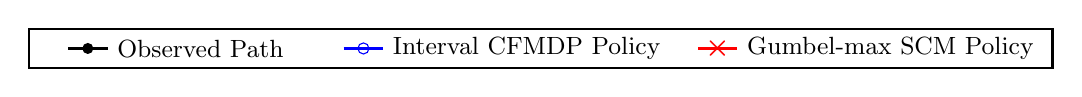
\begin{tikzpicture}[scale=1.0, every node/.style={scale=1.0}]
            \draw[thick, black] (-3, -0.25) rectangle (10, 0.25);
            %
            \draw[black, line width=1pt] (-2.5, 0.0) -- (-2,0.0);
            \fill[black] (-2.25,0.0) circle (2pt); %
            \node[right] at (-2,0.0) {\small Observed Path};
            
            %
            \draw[blue, line width=1pt] (1.0,0.0) -- (1.5,0.0);
            \node[draw=blue, circle, minimum size=4pt, inner sep=0pt] at (1.25,0.0) {}; %
            \node[right] at (1.5,0.0) {\small Interval CFMDP Policy};
            
            %
            \draw[red, line width=1pt] (5.5,0) -- (6,0);
            \node[red] at (5.75,0) {$\boldsymbol{\times}$}; %
            \node[right] at (6,0) {\small Gumbel-max SCM Policy};
        \end{tikzpicture}
    }\\
    %
    \subfigure[\footnotesize Lowest cumulative reward: Interval CFMDP ($312$), Gumbel-max SCM ($312$)]{%
        \resizebox{0.76\columnwidth}{!}{
             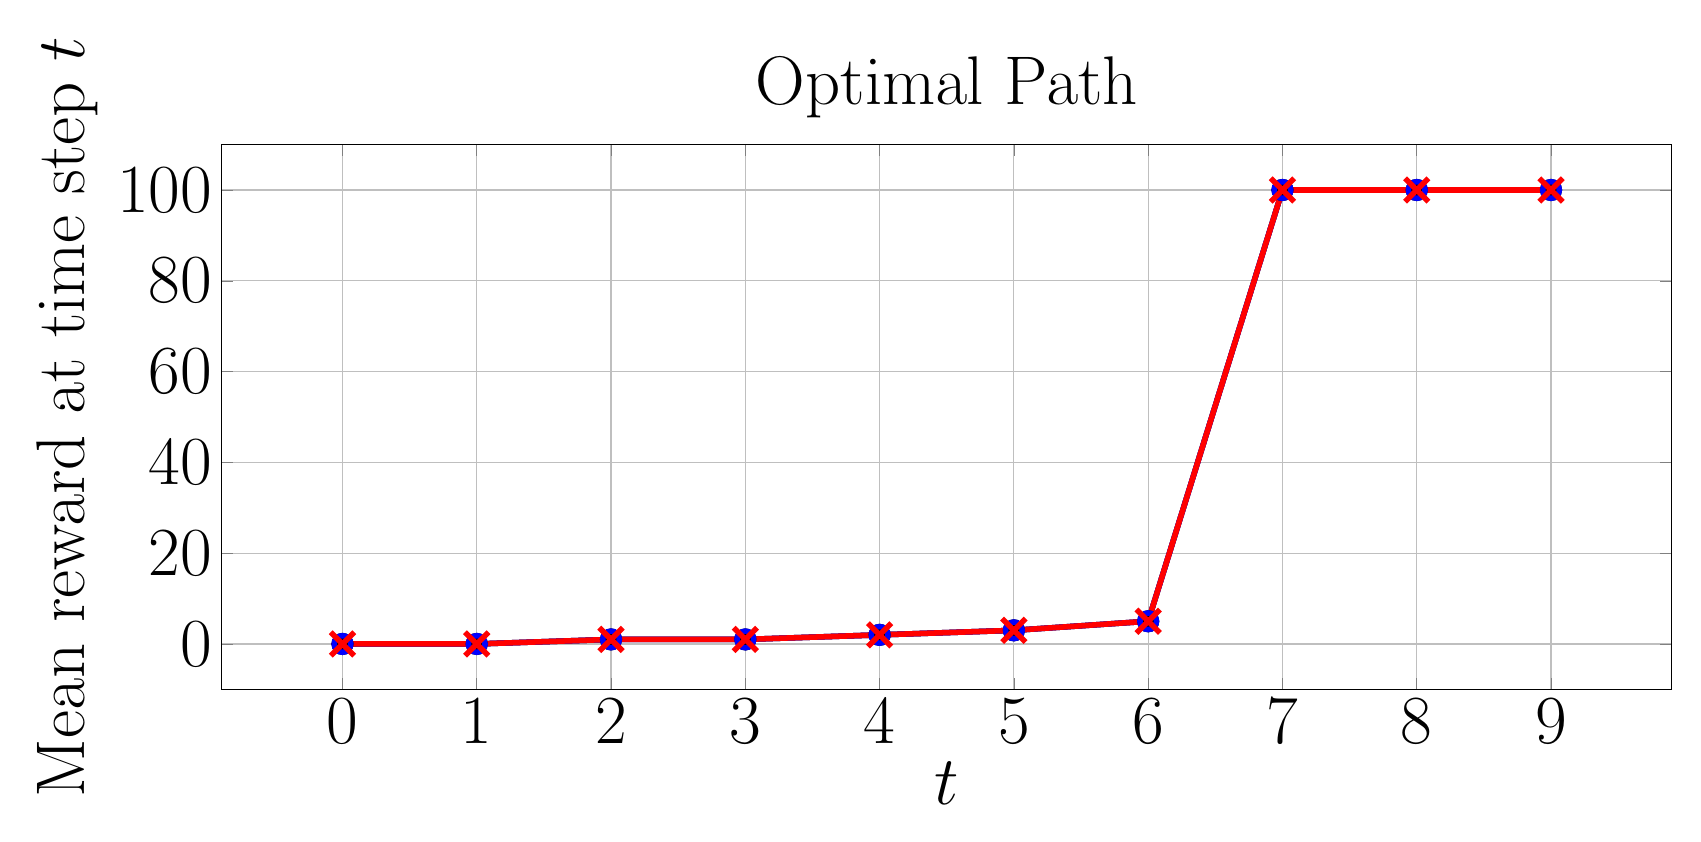
\begin{tikzpicture}
                \begin{axis}[
                    xlabel={$t$},
                    ylabel={Mean reward at time step $t$},
                    title={Optimal Path},
                    grid=both,
                    width=20cm, height=8.5cm,
                    every axis/.style={font=\Huge},
                    %
                ]
                \addplot[
                    color=black, %
                    mark=*, %
                    line width=2pt,
                    mark size=3pt,
                    error bars/.cd,
                    y dir=both, %
                    y explicit, %
                    error bar style={line width=1pt,solid},
                    error mark options={line width=1pt,mark size=4pt,rotate=90}
                ]
                coordinates {
                    (0, 0.0)  +- (0, 0.0)
                    (1, 0.0)  +- (0, 0.0) 
                    (2, 1.0)  +- (0, 0.0) 
                    (3, 1.0)  +- (0, 0.0)
                    (4, 2.0)  +- (0, 0.0)
                    (5, 3.0) +- (0, 0.0)
                    (6, 5.0) +- (0, 0.0)
                    (7, 100.0) +- (0, 0.0)
                    (8, 100.0) +- (0, 0.0)
                    (9, 100.0) +- (0, 0.0)
                };
                %
                \addplot[
                    color=blue, %
                    mark=o, %
                    line width=2pt,
                    mark size=3pt,
                    error bars/.cd,
                    y dir=both, %
                    y explicit, %
                    error bar style={line width=1pt,solid},
                    error mark options={line width=1pt,mark size=4pt,rotate=90}
                ]
                 coordinates {
                    (0, 0.0)  +- (0, 0.0)
                    (1, 0.0)  +- (0, 0.0) 
                    (2, 1.0)  +- (0, 0.0) 
                    (3, 1.0)  +- (0, 0.0)
                    (4, 2.0)  +- (0, 0.0)
                    (5, 3.0) +- (0, 0.0)
                    (6, 5.0) +- (0, 0.0)
                    (7, 100.0) +- (0, 0.0)
                    (8, 100.0) +- (0, 0.0)
                    (9, 100.0) +- (0, 0.0)
                };
                %
                \addplot[
                    color=red, %
                    mark=x, %
                    line width=2pt,
                    mark size=6pt,
                    error bars/.cd,
                    y dir=both, %
                    y explicit, %
                    error bar style={line width=1pt,solid},
                    error mark options={line width=1pt,mark size=4pt,rotate=90}
                ]
                coordinates {
                    (0, 0.0)  +- (0, 0.0)
                    (1, 0.0)  +- (0, 0.0) 
                    (2, 1.0)  +- (0, 0.0) 
                    (3, 1.0)  +- (0, 0.0)
                    (4, 2.0)  +- (0, 0.0)
                    (5, 3.0) +- (0, 0.0)
                    (6, 5.0) +- (0, 0.0)
                    (7, 100.0) +- (0, 0.0)
                    (8, 100.0) +- (0, 0.0)
                    (9, 100.0) +- (0, 0.0)
                };
                \end{axis}
            \end{tikzpicture}
         }
    }
    \hspace{1cm}
    \subfigure[\footnotesize Lowest cumulative reward: Interval CFMDP ($19$), Gumbel-max SCM ($-88$)]{%
         \resizebox{0.76\columnwidth}{!}{
            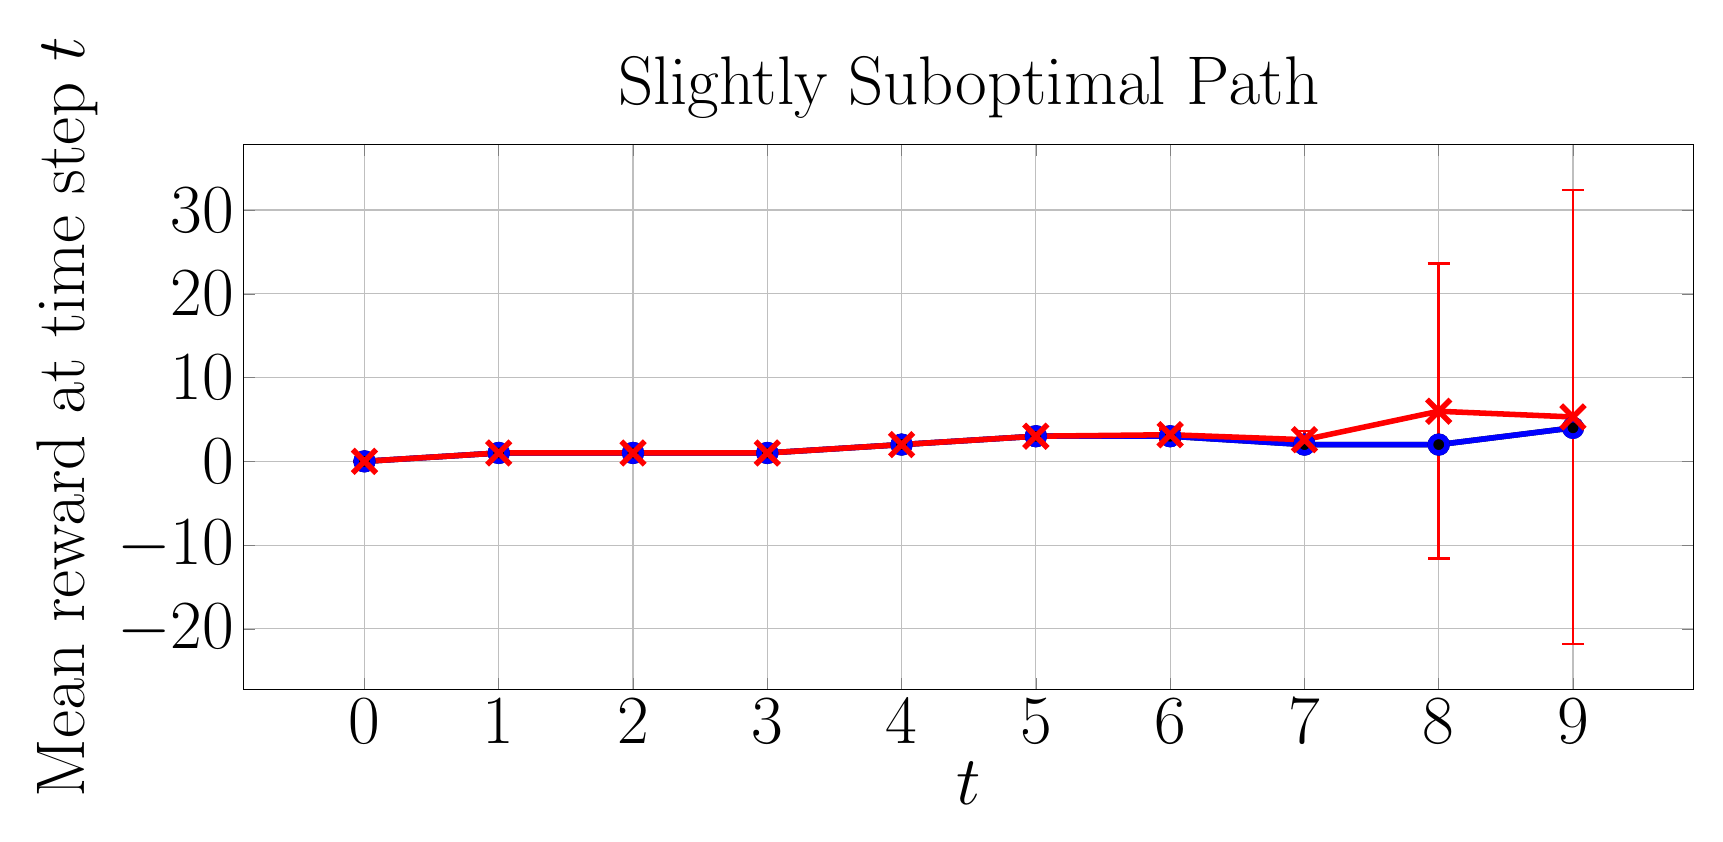
\begin{tikzpicture}
                \begin{axis}[
                    xlabel={$t$},
                    ylabel={Mean reward at time step $t$},
                    title={Slightly Suboptimal Path},
                    grid=both,
                    width=20cm, height=8.5cm,
                    every axis/.style={font=\Huge},
                    %
                ]
                \addplot[
                    color=black, %
                    mark=*, %
                    line width=2pt,
                    mark size=3pt,
                    error bars/.cd,
                    y dir=both, %
                    y explicit, %
                    error bar style={line width=1pt,solid},
                    error mark options={line width=1pt,mark size=4pt,rotate=90}
                ]
              coordinates {
                    (0, 0.0)  +- (0, 0.0)
                    (1, 1.0)  +- (0, 0.0) 
                    (2, 1.0)  +- (0, 0.0) 
                    (3, 1.0)  +- (0, 0.0)
                    (4, 2.0)  +- (0, 0.0)
                    (5, 3.0) +- (0, 0.0)
                    (6, 3.0) +- (0, 0.0)
                    (7, 2.0) +- (0, 0.0)
                    (8, 2.0) +- (0, 0.0)
                    (9, 4.0) +- (0, 0.0)
                };
                %
                \addplot[
                    color=blue, %
                    mark=o, %
                    line width=2pt,
                    mark size=3pt,
                    error bars/.cd,
                    y dir=both, %
                    y explicit, %
                    error bar style={line width=1pt,solid},
                    error mark options={line width=1pt,mark size=4pt,rotate=90}
                ]
              coordinates {
                    (0, 0.0)  +- (0, 0.0)
                    (1, 1.0)  +- (0, 0.0) 
                    (2, 1.0)  +- (0, 0.0) 
                    (3, 1.0)  +- (0, 0.0)
                    (4, 2.0)  +- (0, 0.0)
                    (5, 3.0) +- (0, 0.0)
                    (6, 3.0) +- (0, 0.0)
                    (7, 2.0) +- (0, 0.0)
                    (8, 2.0) +- (0, 0.0)
                    (9, 4.0) +- (0, 0.0)
                };
                %
                \addplot[
                    color=red, %
                    mark=x, %
                    line width=2pt,
                    mark size=6pt,
                    error bars/.cd,
                    y dir=both, %
                    y explicit, %
                    error bar style={line width=1pt,solid},
                    error mark options={line width=1pt,mark size=4pt,rotate=90}
                ]
                coordinates {
                    (0, 0.0)  +- (0, 0.0)
                    (1, 1.0)  +- (0, 0.0) 
                    (2, 1.0)  +- (0, 0.0) 
                    (3, 1.0)  +- (0, 0.0)
                    (4, 2.0)  += (0, 0.0)
                    (5, 3.0)  += (0, 0.0)
                    (6, 3.17847) += (0, 0.62606746) -= (0, 0.62606746)
                    (7, 2.5832885) += (0, 1.04598233) -= (0, 1.04598233)
                    (8, 5.978909) += (0, 17.60137623) -= (0, 17.60137623)
                    (9, 5.297059) += (0, 27.09227512) -= (0, 27.09227512)
                };
                \end{axis}
            \end{tikzpicture}
         }
    }\\[-1.5pt]
    \subfigure[\footnotesize Lowest cumulative reward: Interval CFMDP ($14$), Gumbel-max SCM ($-598$)]{%
         \resizebox{0.76\columnwidth}{!}{
             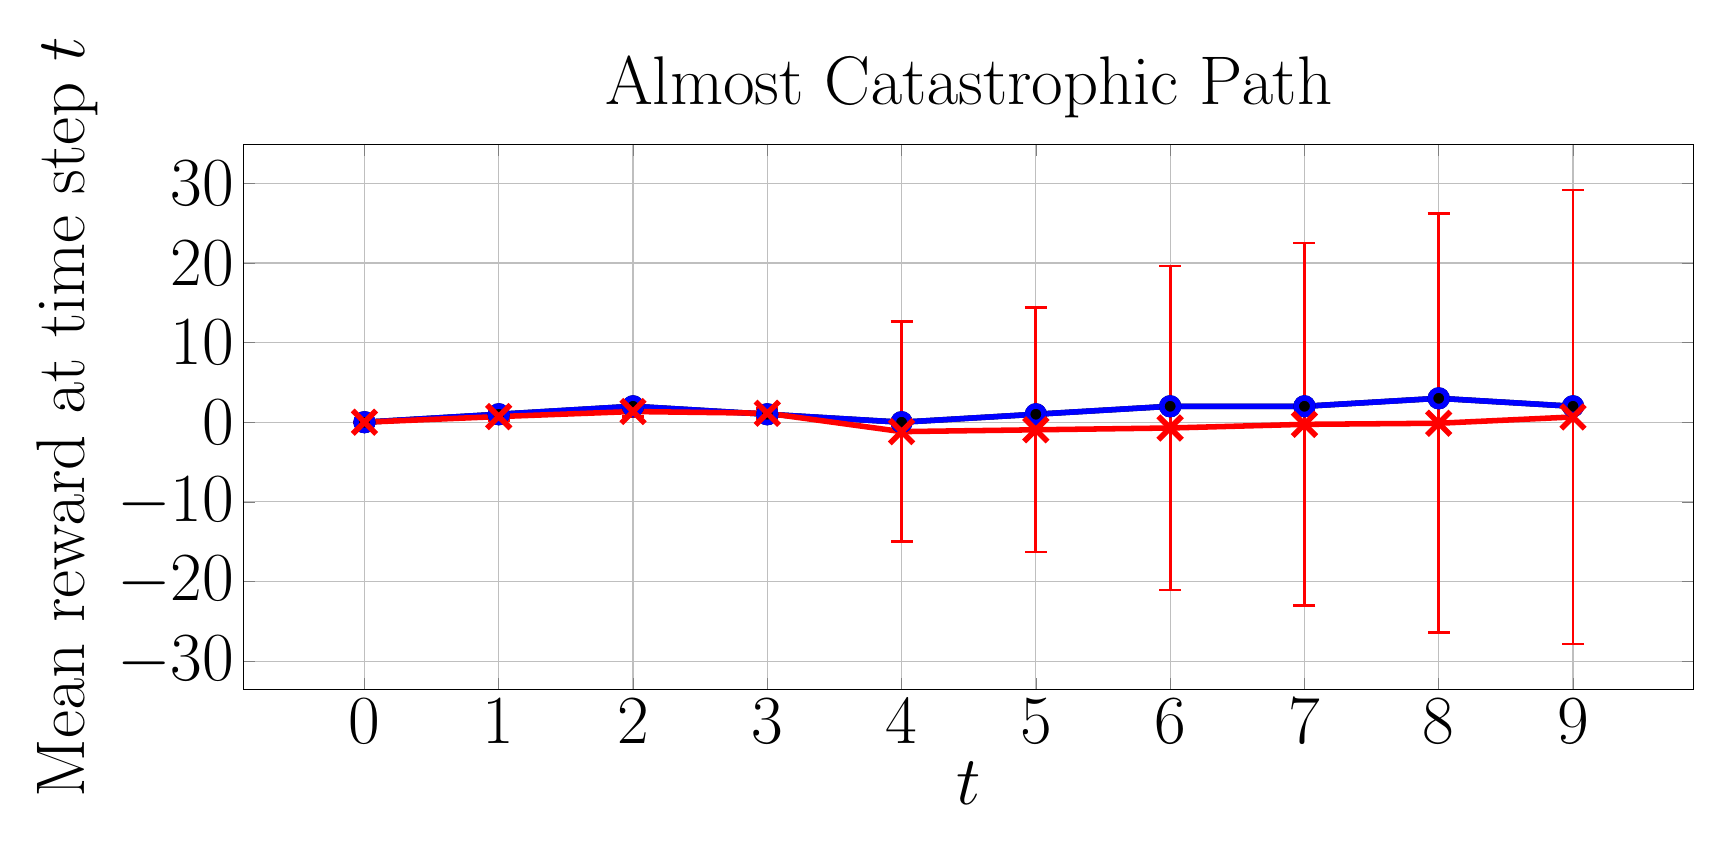
\begin{tikzpicture}
                \begin{axis}[
                    xlabel={$t$},
                    ylabel={Mean reward at time step $t$},
                    title={Almost Catastrophic Path},
                    grid=both,
                    width=20cm, height=8.5cm,
                    every axis/.style={font=\Huge},
                    %
                ]
                \addplot[
                    color=black, %
                    mark=*, %
                    line width=2pt,
                    mark size=3pt,
                    error bars/.cd,
                    y dir=both, %
                    y explicit, %
                    error bar style={line width=1pt,solid},
                    error mark options={line width=1pt,mark size=4pt,rotate=90}
                ]
                coordinates {
                    (0, 0.0)  +- (0, 0.0)
                    (1, 1.0)  +- (0, 0.0) 
                    (2, 2.0)  +- (0, 0.0) 
                    (3, 1.0)  +- (0, 0.0)
                    (4, 0.0)  +- (0, 0.0)
                    (5, 1.0) +- (0, 0.0)
                    (6, 2.0) +- (0, 0.0)
                    (7, 2.0) +- (0, 0.0)
                    (8, 3.0) +- (0, 0.0)
                    (9, 2.0) +- (0, 0.0)
                };
                %
                \addplot[
                    color=blue, %
                    mark=o, %
                    line width=2pt,
                    mark size=3pt,
                    error bars/.cd,
                    y dir=both, %
                    y explicit, %
                    error bar style={line width=1pt,solid},
                    error mark options={line width=1pt,mark size=4pt,rotate=90}
                ]
                coordinates {
                    (0, 0.0)  +- (0, 0.0)
                    (1, 1.0)  +- (0, 0.0) 
                    (2, 2.0)  +- (0, 0.0) 
                    (3, 1.0)  +- (0, 0.0)
                    (4, 0.0)  +- (0, 0.0)
                    (5, 1.0) +- (0, 0.0)
                    (6, 2.0) +- (0, 0.0)
                    (7, 2.0) +- (0, 0.0)
                    (8, 3.0) +- (0, 0.0)
                    (9, 2.0) +- (0, 0.0)
                };
                %
                \addplot[
                    color=red, %
                    mark=x, %
                    line width=2pt,
                    mark size=6pt,
                    error bars/.cd,
                    y dir=both, %
                    y explicit, %
                    error bar style={line width=1pt,solid},
                    error mark options={line width=1pt,mark size=4pt,rotate=90}
                ]
                coordinates {
                    (0, 0.0)  +- (0, 0.0)
                    (1, 0.7065655)  +- (0, 0.4553358) 
                    (2, 1.341673)  +- (0, 0.67091621) 
                    (3, 1.122926)  +- (0, 0.61281824)
                    (4, -1.1821935)  +- (0, 13.82444042)
                    (5, -0.952399)  +- (0, 15.35195457)
                    (6, -0.72672) +- (0, 20.33508414)
                    (7, -0.268983) +- (0, 22.77861454)
                    (8, -0.1310835) +- (0, 26.31013314)
                    (9, 0.65806) +- (0, 28.50670214)
                };
                %
            %
            %
            %
            %
            %
            %
            %
            %
            %
            %
            %
            %
            %
            %
            %
            %
            %
            %
                \end{axis}
            \end{tikzpicture}
         }
    }
    \hspace{1cm}
    \subfigure[\footnotesize Lowest cumulative reward: Interval CFMDP ($-698$), Gumbel-max SCM ($-698$)]{%
         \resizebox{0.76\columnwidth}{!}{
            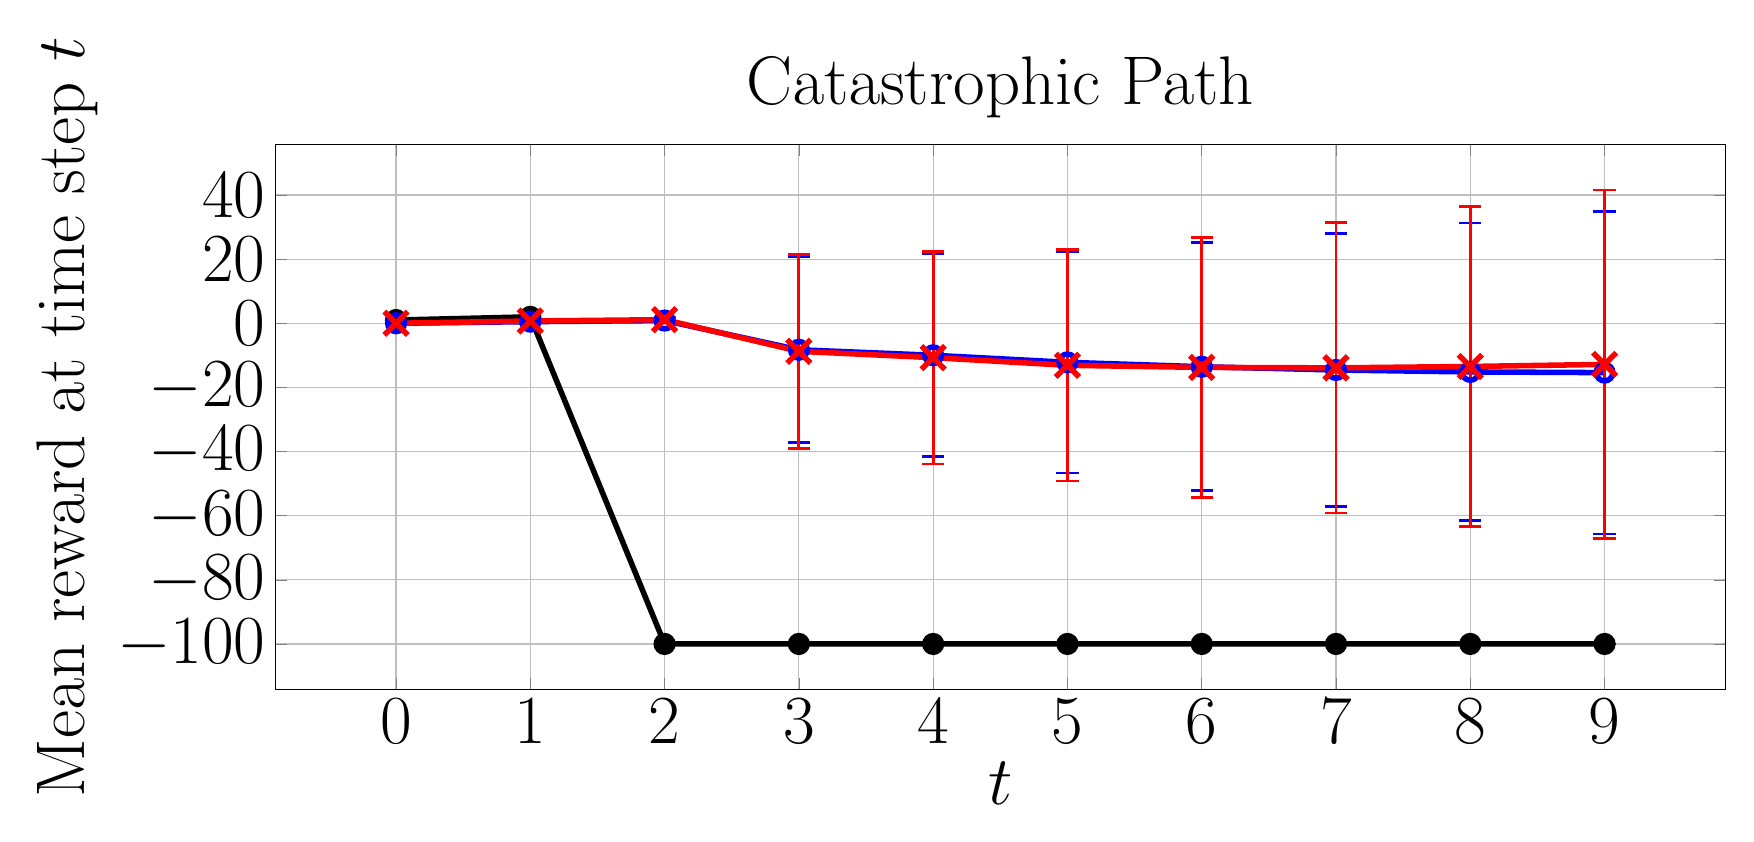
\begin{tikzpicture}
                \begin{axis}[
                    xlabel={$t$},
                    ylabel={Mean reward at time step $t$},
                    title={Catastrophic Path},
                    grid=both,
                    width=20cm, height=8.5cm,
                    every axis/.style={font=\Huge},
                    %
                ]
                \addplot[
                    color=black, %
                    mark=*, %
                    line width=2pt,
                    mark size=3pt,
                    error bars/.cd,
                    y dir=both, %
                    y explicit, %
                    error bar style={line width=1pt,solid},
                    error mark options={line width=1pt,mark size=4pt,rotate=90}
                ]
                coordinates {
                    (0, 1.0)  +- (0, 0.0)
                    (1, 2.0)  +- (0, 0.0) 
                    (2, -100.0)  +- (0, 0.0) 
                    (3, -100.0)  +- (0, 0.0)
                    (4, -100.0)  +- (0, 0.0)
                    (5, -100.0) +- (0, 0.0)
                    (6, -100.0) +- (0, 0.0)
                    (7, -100.0) +- (0, 0.0)
                    (8, -100.0) +- (0, 0.0)
                    (9, -100.0) +- (0, 0.0)
                };
                %
                \addplot[
                    color=blue, %
                    mark=o, %
                    line width=2pt,
                    mark size=3pt,
                    error bars/.cd,
                    y dir=both, %
                    y explicit, %
                    error bar style={line width=1pt,solid},
                    error mark options={line width=1pt,mark size=4pt,rotate=90}
                ]
                coordinates {
                    (0, 0.0)  +- (0, 0.0)
                    (1, 0.504814)  +- (0, 0.49997682) 
                    (2, 0.8439835)  +- (0, 0.76831917) 
                    (3, -8.2709165)  +- (0, 28.93656754)
                    (4, -9.981082)  +- (0, 31.66825363)
                    (5, -12.1776325) +- (0, 34.53463233)
                    (6, -13.556076) +- (0, 38.62845372)
                    (7, -14.574418) +- (0, 42.49603359)
                    (8, -15.1757075) +- (0, 46.41913968)
                    (9, -15.3900395) +- (0, 50.33563368)
                };
                %
                \addplot[
                    color=red, %
                    mark=x, %
                    line width=2pt,
                    mark size=6pt,
                    error bars/.cd,
                    y dir=both, %
                    y explicit, %
                    error bar style={line width=1pt,solid},
                    error mark options={line width=1pt,mark size=4pt,rotate=90}
                ]
                coordinates {
                    (0, 0.0)  +- (0, 0.0)
                    (1, 0.701873)  +- (0, 0.45743556) 
                    (2, 1.1227805)  +- (0, 0.73433129) 
                    (3, -8.7503255)  +- (0, 30.30257976)
                    (4, -10.722092)  +- (0, 33.17618589)
                    (5, -13.10721)  +- (0, 36.0648089)
                    (6, -13.7631645) +- (0, 40.56553451)
                    (7, -13.909043) +- (0, 45.23829402)
                    (8, -13.472517) +- (0, 49.96270296)
                    (9, -12.8278835) +- (0, 54.38618735)
                };
                %
            %
            %
            %
            %
            %
            %
            %
            %
            %
            %
            %
            %
            %
            %
            %
            %
            %
            %
                \end{axis}
            \end{tikzpicture}
         }
    }
    \caption{Average instant reward of CF paths induced by policies on GridWorld $p=0.4$.}
    \label{fig: reward p=0.4}
\end{figure*}

\subsection{Experimental Setup}
To compare policy performance, we measure the average rewards of counterfactual paths induced by our policy and the Gumbel-max policy by uniformly sampling $200$ counterfactual MDPs from the ICFMDP and generating $10,000$ counterfactual paths over each sampled CFMDP. \jl{Since the interval CFMDP depends on the observed path, we select $4$  paths of varying optimality to evaluate how the observed path impacts the performance of both policies: an optimal path, a slightly suboptimal path that could reach the optimal reward with a few changes, a catastrophic path that enters a catastrophic, terminal state with low reward, and an almost catastrophic path that was close to entering a catastrophic state.} When measuring the average probability bound widths and execution time needed to generate the ICFMDPs, we averaged over $20$ randomly generated observed paths
\footnote{Further training details are provided in Appendix \ref{app: training details}, and the code is provided at \href{https://github.com/ddv-lab/robust-cf-inference-in-MDPs}{https://github.com/ddv-lab/robust-cf-inference-in-MDPs}
%
%
.}.

\subsection{GridWorld}
\jl{The GridWorld MDP is a $4 \times 4$ grid where an agent must navigate from the top-left corner to the goal state in the bottom-right corner, avoiding a dangerous terminal state in the centre. At each time step, the agent can move up, down, left, or right, but there is a small probability (controlled by hyper-parameter $p$) of moving in an unintended direction. As the agent nears the goal, the reward for each state increases, culminating in a reward of $+100$ for reaching the goal. Entering the dangerous state results in a penalty of $-100$. We use two versions of GridWorld: a less stochastic version with $p=0.9$ (i.e., $90$\% chance of moving in the chosen direction) and a more stochastic version with $p=0.4$.}

\paragraph{GridWorld ($p=0.9$)}
When $p=0.9$, the counterfactual probability bounds are typically narrow (see Table \ref{tab:nonzero_probs} for average measurements). Consequently, as shown in Figure \ref{fig: reward p=0.9}, both policies are nearly identical and perform similarly well across the optimal, slightly suboptimal, and catastrophic paths.
%
However, for the almost catastrophic path, the interval CFMDP path is more conservative and follows the observed path more closely (as this is where the probability bounds are narrowest), which typically requires one additional step to reach the goal state than the Gumbel-max SCM policy.
%

\paragraph{GridWorld ($p=0.4$)}
\jl{When $p=0.4$, the GridWorld environment becomes more uncertain, increasing the risk of entering the dangerous state even if correct actions are chosen. Thus, as shown in Figure \ref{fig: reward p=0.4}, the interval CFMDP policy adopts a more conservative approach, avoiding deviation from the observed policy if it cannot guarantee higher counterfactual rewards (see the slightly suboptimal and almost catastrophic paths), whereas the Gumbel-max SCM is inconsistent: it can yield higher rewards, but also much lower rewards, reflected in the wide error bars.} For the catastrophic path, both policies must deviate from the observed path to achieve a higher reward and, in this case, perform similarly.
%
%
%
%
\subsection{Sepsis}
The Sepsis MDP \citep{oberst2019counterfactual} simulates trajectories of Sepsis patients. Each state consists of four vital signs (heart rate, blood pressure, oxygen concentration, and glucose levels), categorised as low, normal, or high.
and three treatments that can be toggled on/off at each time step (8 actions in total). Unlike \citet{oberst2019counterfactual}, we scale rewards based on the number of out-of-range vital signs, between $-1000$ (patient dies) and $1000$ (patient discharged). \jl{Like the GridWorld $p=0.4$ experiment, the Sepsis MDP is highly uncertain, as many states are equally likely to lead to optimal and poor outcomes. Thus, as shown in Figure \ref{fig: reward sepsis}, both policies follow the observed optimal and almost catastrophic paths to guarantee rewards are no worse than the observation.} However, improving the catastrophic path requires deviating from the observation. Here, the Gumbel-max SCM policy, on average, performs better than the interval CFMDP policy. But, since both policies have lower bounds clipped at $-1000$, neither policy reliably improves over the observation. In contrast, for the slightly suboptimal path, the interval CFMDP policy performs significantly better, shown by its higher lower bounds. 
Moreover, in these two cases, the worst-case counterfactual path generated by the interval CFMDP policy is better than that of the Gumbel-max SCM policy,
indicating its greater robustness.
%
\begin{figure*}
    \centering
     \resizebox{0.6\textwidth}{!}{
        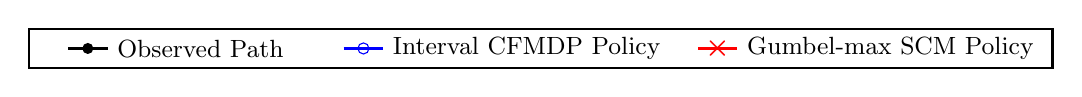
\begin{tikzpicture}[scale=1.0, every node/.style={scale=1.0}]
            \draw[thick, black] (-3, -0.25) rectangle (10, 0.25);
            %
            \draw[black, line width=1pt] (-2.5, 0.0) -- (-2,0.0);
            \fill[black] (-2.25,0.0) circle (2pt); %
            \node[right] at (-2,0.0) {\small Observed Path};
            
            %
            \draw[blue, line width=1pt] (1.0,0.0) -- (1.5,0.0);
            \node[draw=blue, circle, minimum size=4pt, inner sep=0pt] at (1.25,0.0) {}; %
            \node[right] at (1.5,0.0) {\small Interval CFMDP Policy};
            
            %
            \draw[red, line width=1pt] (5.5,0) -- (6,0);
            \node[red] at (5.75,0) {$\boldsymbol{\times}$}; %
            \node[right] at (6,0) {\small Gumbel-max SCM Policy};
        \end{tikzpicture}
    }\\
    \subfigure[\footnotesize Lowest cumulative reward: Interval CFMDP ($8000$), Gumbel-max SCM ($8000$)]{%
         \resizebox{0.76\columnwidth}{!}{
             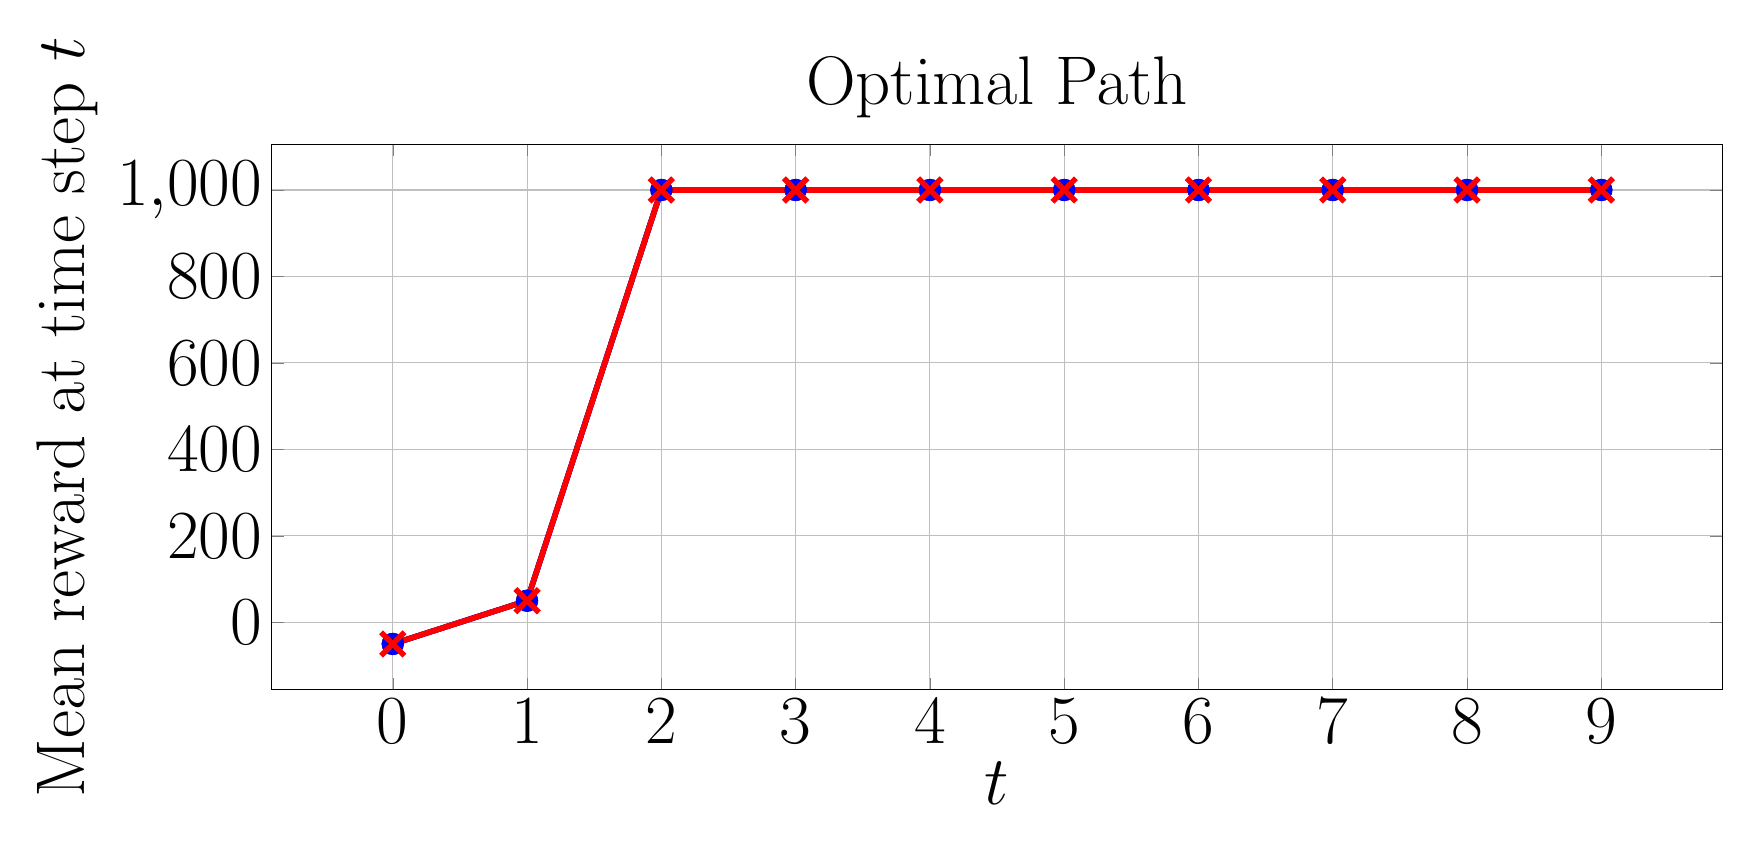
\begin{tikzpicture}
                \begin{axis}[
                    xlabel={$t$},
                    ylabel={Mean reward at time step $t$},
                    title={Optimal Path},
                    grid=both,
                    width=20cm, height=8.5cm,
                    every axis/.style={font=\Huge},
                    %
                ]
                \addplot[
                    color=black, %
                    mark=*, %
                    line width=2pt,
                    mark size=3pt,
                ]
                coordinates {
                    (0, -50.0)
                    (1, 50.0)
                    (2, 1000.0)
                    (3, 1000.0)
                    (4, 1000.0)
                    (5, 1000.0)
                    (6, 1000.0)
                    (7, 1000.0)
                    (8, 1000.0)
                    (9, 1000.0)
                };
                %
                \addplot[
                    color=blue, %
                    mark=o, %
                    line width=2pt,
                    mark size=3pt,
                    error bars/.cd,
                    y dir=both, %
                    y explicit, %
                    error bar style={line width=1pt,solid},
                    error mark options={line width=1pt,mark size=4pt,rotate=90}
                ]
                coordinates {
                    (0, -50.0)  +- (0, 0.0)
                    (1, 50.0)  +- (0, 0.0) 
                    (2, 1000.0)  +- (0, 0.0) 
                    (3, 1000.0)  +- (0, 0.0)
                    (4, 1000.0)  +- (0, 0.0)
                    (5, 1000.0) +- (0, 0.0)
                    (6, 1000.0) +- (0, 0.0)
                    (7, 1000.0) +- (0, 0.0)
                    (8, 1000.0) +- (0, 0.0)
                    (9, 1000.0) +- (0, 0.0)
                };
                %
                \addplot[
                    color=red, %
                    mark=x, %
                    line width=2pt,
                    mark size=6pt,
                    error bars/.cd,
                    y dir=both, %
                    y explicit, %
                    error bar style={line width=1pt,solid},
                    error mark options={line width=1pt,mark size=4pt,rotate=90}
                ]
                coordinates {
                    (0, -50.0)  +- (0, 0.0)
                    (1, 50.0)  +- (0, 0.0) 
                    (2, 1000.0)  +- (0, 0.0) 
                    (3, 1000.0)  +- (0, 0.0)
                    (4, 1000.0)  +- (0, 0.0)
                    (5, 1000.0) +- (0, 0.0)
                    (6, 1000.0) +- (0, 0.0)
                    (7, 1000.0) +- (0, 0.0)
                    (8, 1000.0) +- (0, 0.0)
                    (9, 1000.0) +- (0, 0.0)
                };
                %
                \end{axis}
            \end{tikzpicture}
         }
    }
    \hspace{1cm}
    \subfigure[\footnotesize Lowest cumulative reward: Interval CFMDP ($-5980$), Gumbel-max SCM ($-8000$)]{%
         \resizebox{0.76\columnwidth}{!}{
            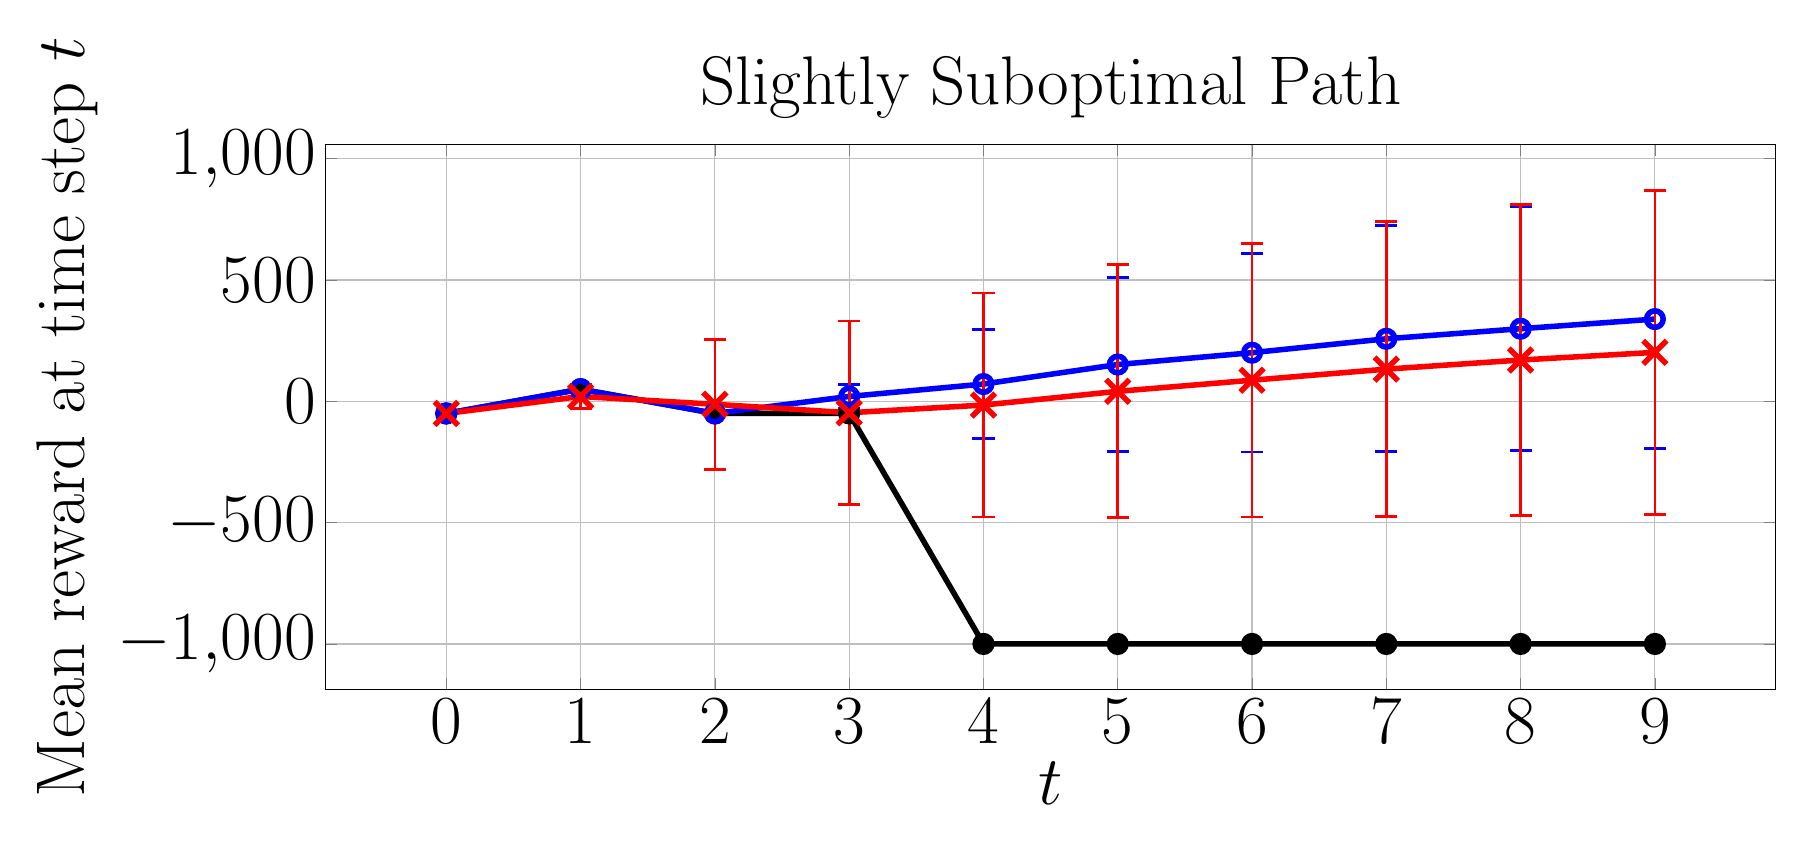
\begin{tikzpicture}
                \begin{axis}[
                    xlabel={$t$},
                    ylabel={Mean reward at time step $t$},
                    title={Slightly Suboptimal Path},
                    grid=both,
                    width=20cm, height=8.5cm,
                    every axis/.style={font=\Huge},
                    %
                ]
               \addplot[
                    color=black, %
                    mark=*, %
                    line width=2pt,
                    mark size=3pt,
                ]
                coordinates {
                    (0, -50.0)
                    (1, 50.0)
                    (2, -50.0)
                    (3, -50.0)
                    (4, -1000.0)
                    (5, -1000.0)
                    (6, -1000.0)
                    (7, -1000.0)
                    (8, -1000.0)
                    (9, -1000.0)
                };
                %
                \addplot[
                    color=blue, %
                    mark=o, %
                    line width=2pt,
                    mark size=3pt,
                    error bars/.cd,
                    y dir=both, %
                    y explicit, %
                    error bar style={line width=1pt,solid},
                    error mark options={line width=1pt,mark size=4pt,rotate=90}
                ]
                coordinates {
                    (0, -50.0)  +- (0, 0.0)
                    (1, 50.0)  +- (0, 0.0) 
                    (2, -50.0)  +- (0, 0.0) 
                    (3, 20.0631)  +- (0, 49.97539413)
                    (4, 71.206585)  +- (0, 226.02033693)
                    (5, 151.60797) +- (0, 359.23292559)
                    (6, 200.40593) +- (0, 408.86185176)
                    (7, 257.77948) +- (0, 466.10372804)
                    (8, 299.237465) +- (0, 501.82579506)
                    (9, 338.9129) +- (0, 532.06124996)
                };
                %
                \addplot[
                    color=red, %
                    mark=x, %
                    line width=2pt,
                    mark size=6pt,
                    error bars/.cd,
                    y dir=both, %
                    y explicit, %
                    error bar style={line width=1pt,solid},
                    error mark options={line width=1pt,mark size=4pt,rotate=90}
                ]
                coordinates {
                    (0, -50.0)  +- (0, 0.0)
                    (1, 20.00736)  +- (0, 49.99786741) 
                    (2, -12.282865)  +- (0, 267.598755) 
                    (3, -47.125995)  +- (0, 378.41755832)
                    (4, -15.381965)  +- (0, 461.77616558)
                    (5, 41.15459) +- (0, 521.53189262)
                    (6, 87.01595) +- (0, 564.22243126 )
                    (7, 132.62376) +- (0, 607.31338037)
                    (8, 170.168145) +- (0, 641.48013693)
                    (9, 201.813135) +- (0, 667.29441777)
                };
                %
                %
                %
                %
                %
                %
                %
                %
                %
                %
                %
                %
                %
                %
                %
                %
                %
                %
                %
                \end{axis}
            \end{tikzpicture}
         }
    }\\[-1.5pt]
    \subfigure[\footnotesize Lowest cumulative reward: Interval CFMDP ($100$), Gumbel-max SCM ($100$)]{%
         \resizebox{0.76\columnwidth}{!}{
             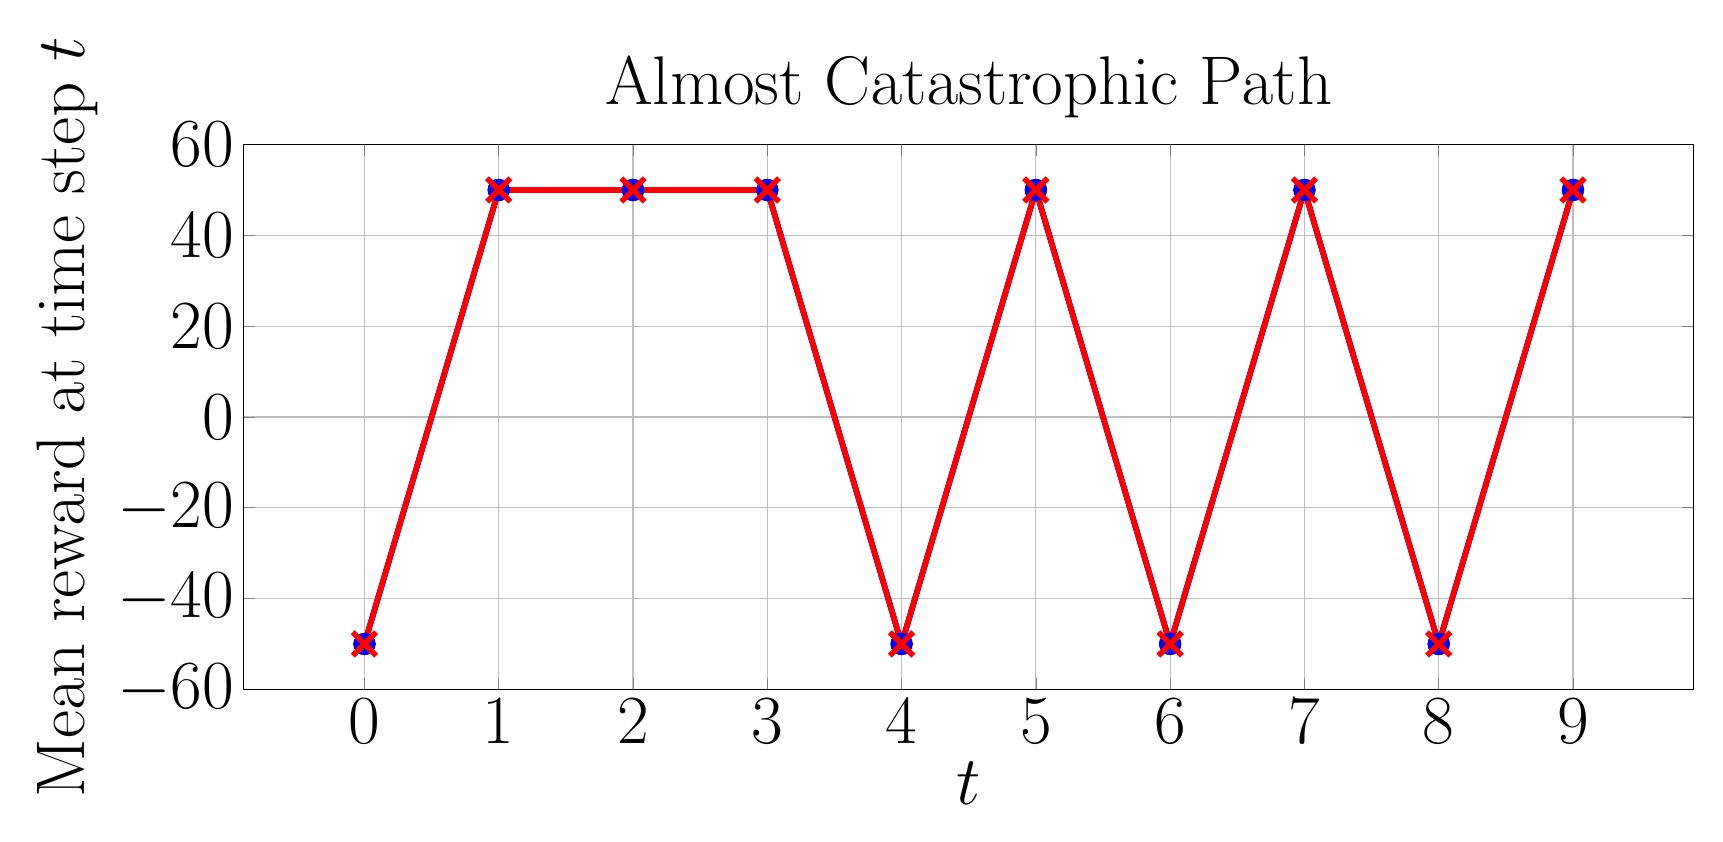
\begin{tikzpicture}
                \begin{axis}[
                    xlabel={$t$},
                    ylabel={Mean reward at time step $t$},
                    title={Almost Catastrophic Path},
                    grid=both,
                    every axis/.style={font=\Huge},
                    width=20cm, height=8.5cm,
                    %
                ]
               \addplot[
                    color=black, %
                    mark=*, %
                    line width=2pt,
                    mark size=3pt,
                ]
                coordinates {
                    (0, -50.0)
                    (1, 50.0)
                    (2, 50.0)
                    (3, 50.0)
                    (4, -50.0)
                    (5, 50.0)
                    (6, -50.0)
                    (7, 50.0)
                    (8, -50.0)
                    (9, 50.0)
                };
                %
                %
                \addplot[
                    color=blue, %
                    mark=o, %
                    line width=2pt,
                    mark size=3pt,
                    error bars/.cd,
                    y dir=both, %
                    y explicit, %
                    error bar style={line width=1pt,solid},
                    error mark options={line width=1pt,mark size=4pt,rotate=90}
                ]
                coordinates {
                    (0, -50.0)  +- (0, 0.0)
                    (1, 50.0)  +- (0, 0.0) 
                    (2, 50.0)  +- (0, 0.0) 
                    (3, 50.0)  +- (0, 0.0)
                    (4, -50.0)  +- (0, 0.0)
                    (5, 50.0) +- (0, 0.0)
                    (6, -50.0) +- (0, 0.0)
                    (7, 50.0) +- (0, 0.0)
                    (8, -50.0) +- (0, 0.0)
                    (9, 50.0) +- (0, 0.0)
                };
                %
                \addplot[
                    color=red, %
                    mark=x, %
                    line width=2pt,
                    mark size=6pt,
                    error bars/.cd,
                    y dir=both, %
                    y explicit, %
                    error bar style={line width=1pt,solid},
                    error mark options={line width=1pt,mark size=4pt,rotate=90}
                ]
                coordinates {
                    (0, -50.0)  +- (0, 0.0)
                    (1, 50.0)  +- (0, 0.0) 
                    (2, 50.0)  +- (0, 0.0) 
                    (3, 50.0)  +- (0, 0.0)
                    (4, -50.0)  +- (0, 0.0)
                    (5, 50.0) +- (0, 0.0)
                    (6, -50.0) +- (0, 0.0)
                    (7, 50.0) +- (0, 0.0)
                    (8, -50.0) +- (0, 0.0)
                    (9, 50.0) +- (0, 0.0)
                };
                %
                %
                %
                %
                %
                %
                %
                %
                %
                %
                %
                %
                %
                %
                %
                %
                %
                %
                %
                \end{axis}
            \end{tikzpicture}
         }
    }
    \hspace{1cm}
    \subfigure[\footnotesize Lowest cumulative reward: Interval CFMDP ($-7150$), Gumbel-max SCM ($-9050$)]{%
         \resizebox{0.76\columnwidth}{!}{
            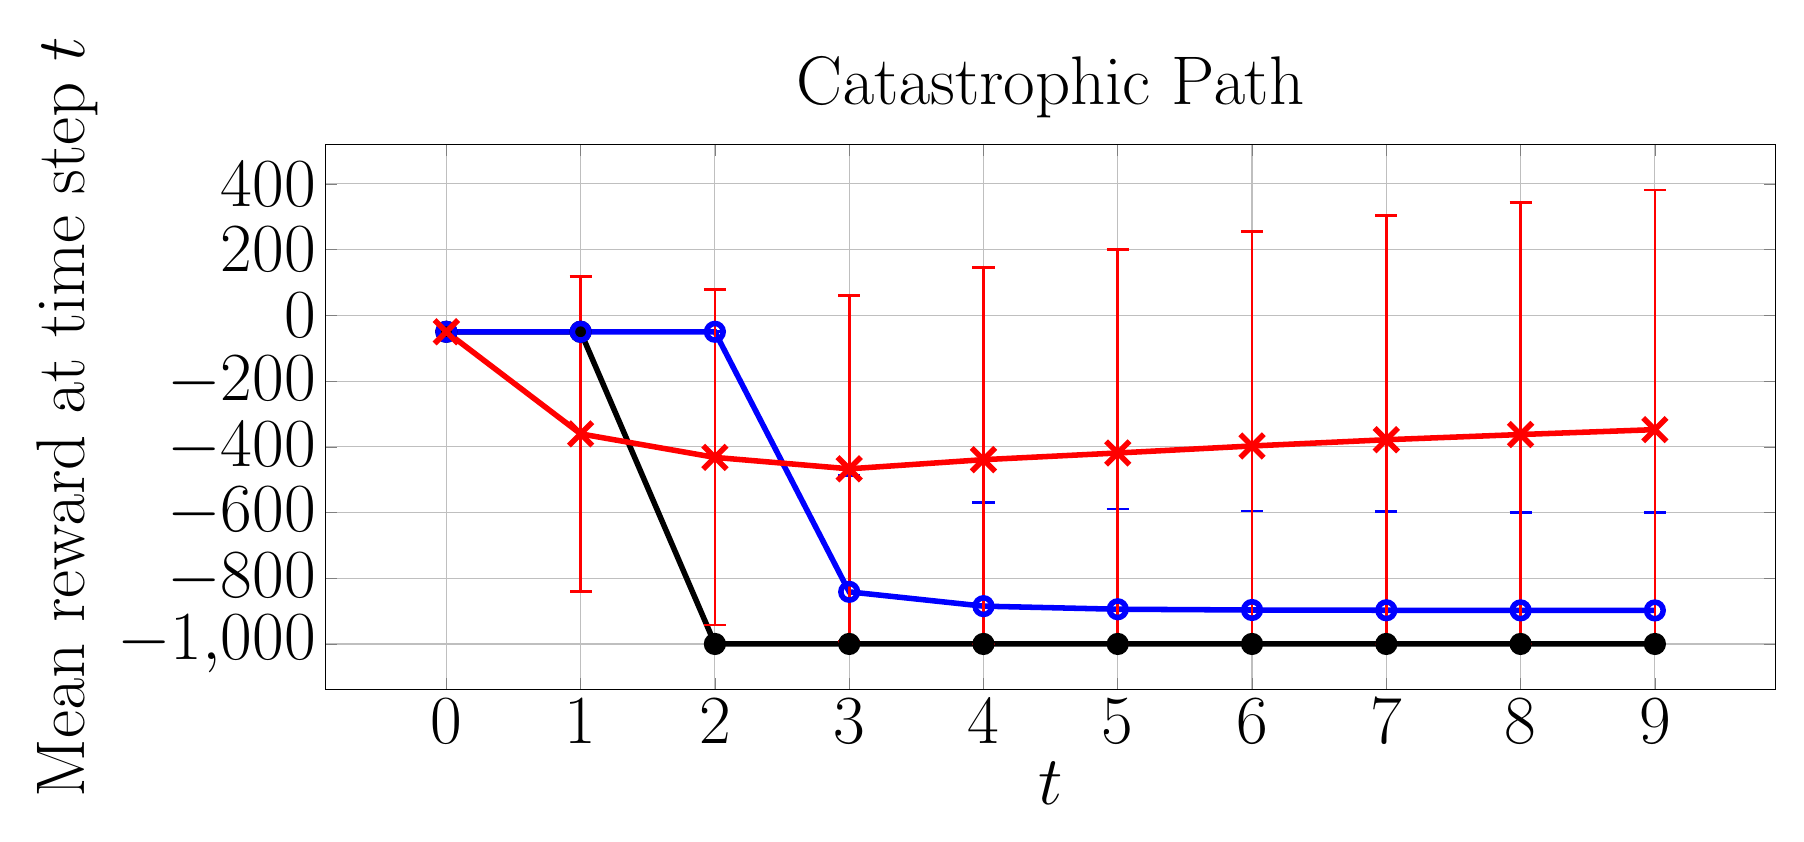
\begin{tikzpicture}
                \begin{axis}[
                    xlabel={$t$},
                    ylabel={Mean reward at time step $t$},
                    title={Catastrophic Path},
                    grid=both,
                    width=20cm, height=8.5cm,
                    every axis/.style={font=\Huge},
                    %
                ]
               \addplot[
                    color=black, %
                    mark=*, %
                    line width=2pt,
                    mark size=3pt,
                ]
                coordinates {
                    (0, -50.0)
                    (1, -50.0)
                    (2, -1000.0)
                    (3, -1000.0)
                    (4, -1000.0)
                    (5, -1000.0)
                    (6, -1000.0)
                    (7, -1000.0)
                    (8, -1000.0)
                    (9, -1000.0)
                };
                %
                %
                \addplot[
                    color=blue, %
                    mark=o, %
                    line width=2pt,
                    mark size=3pt,
                    error bars/.cd,
                    y dir=both, %
                    y explicit, %
                    error bar style={line width=1pt,solid},
                    error mark options={line width=1pt,mark size=4pt,rotate=90}
                ]
                coordinates {
                    (0, -50.0)  +- (0, 0.0)
                    (1, -50.0)  +- (0, 0.0) 
                    (2, -50.0)  +- (0, 0.0) 
                    (3, -841.440725)  += (0, 354.24605512) -= (0, 158.559275)
                    (4, -884.98225)  += (0, 315.37519669) -= (0, 115.01775)
                    (5, -894.330425) += (0, 304.88572805) -= (0, 105.669575)
                    (6, -896.696175) += (0, 301.19954514) -= (0, 103.303825)
                    (7, -897.4635) += (0, 299.61791279) -= (0, 102.5365)
                    (8, -897.77595) += (0, 298.80392585) -= (0, 102.22405)
                    (9, -897.942975) += (0, 298.32920557) -= (0, 102.057025)
                };
                %
                \addplot[
                    color=red, %
                    mark=x, %
                    line width=2pt,
                    mark size=6pt,
                    error bars/.cd,
                    y dir=both, %
                    y explicit, %
                    error bar style={line width=1pt,solid},
                    error mark options={line width=1pt,mark size=4pt,rotate=90}
                ]
            coordinates {
                    (0, -50.0)  +- (0, 0.0)
                    (1, -360.675265)  +- (0, 479.39812699) 
                    (2, -432.27629)  +- (0, 510.38620897) 
                    (3, -467.029545)  += (0, 526.36009628) -= (0, 526.36009628)
                    (4, -439.17429)  += (0, 583.96638919) -= (0, 560.82571)
                    (5, -418.82704) += (0, 618.43027478) -= (0, 581.17296)
                    (6, -397.464895) += (0, 652.67322574) -= (0, 602.535105)
                    (7, -378.49052) += (0, 682.85407033) -= (0, 621.50948)
                    (8, -362.654195) += (0, 707.01412023) -= (0, 637.345805)
                    (9, -347.737935) += (0, 729.29076479) -= (0, 652.262065)
                };
                %
                %
                %
                %
                %
                %
                %
                %
                %
                %
                %
                %
                %
                %
                %
                %
                %
                %
                %
                \end{axis}
            \end{tikzpicture}
         }
    }
    \caption{Average instant reward of CF paths induced by policies on Sepsis.}
    \label{fig: reward sepsis}
\end{figure*}

%
%
%
\subsection{Interval CFMDP Bounds}
%
%
Table \ref{tab:nonzero_probs} presents the mean counterfactual probability bound widths (excluding transitions where the upper bound is $0$) for each MDP, averaged over 20 observed paths. We compare the bounds under counterfactual stability (CS) and monotonicity (M) assumptions, CS alone, and no assumptions. This shows that the assumptions marginally reduce the bound widths, indicating the assumptions tighten the bounds without excluding too many causal models, as intended.
\renewcommand{\arraystretch}{1}

\begin{table}
\centering
\caption{Mean width of counterfactual probability bounds}
\resizebox{0.8\columnwidth}{!}{%
\begin{tabular}{|c|c|c|c|}
\hline
\multirow{2}{*}{\textbf{Environment}} & \multicolumn{3}{c|}{\textbf{Assumptions}} \\ \cline{2-4}
 & \textbf{CS + M} & \textbf{CS} & \textbf{None\tablefootnote{\jl{Equivalent to \citet{li2024probabilities}'s bounds (see Section \ref{sec: equivalence with Li}).}}} \\ \hline
\textbf{GridWorld} ($p=0.9$) & 0.0817 & 0.0977 & 0.100 \\ \hline
\textbf{GridWorld} ($p=0.4$) & 0.552  & 0.638  & 0.646 \\ \hline
\textbf{Sepsis} & 0.138 & 0.140 & 0.140 \\ \hline
\end{tabular}
}
\label{tab:nonzero_probs}
\end{table}


\subsection{Execution Times}
Table \ref{tab: times} compares the average time needed to generate the interval CFMDP vs.\ the Gumbel-max SCM CFMDP for 20 observations.
The GridWorld algorithms were run single-threaded, while the Sepsis experiments were run in parallel.
Generating the interval CFMDP is significantly faster as it uses exact analytical bounds, whereas the Gumbel-max CFMDP requires sampling from the Gumbel distribution to estimate counterfactual transition probabilities. \jl{Since constructing the counterfactual MDP models is the main bottleneck in both approaches, ours is more efficient overall and suitable for larger MDPs.}
\begin{table}
\centering
\caption{Mean execution time to generate CFMDPs}
\resizebox{0.99\columnwidth}{!}{%
\begin{tabular}{|c|c|c|}
\hline
\multirow{2}{*}{\textbf{Environment}} & \multicolumn{2}{c|}{\textbf{Mean Execution Time (s)}} \\ \cline{2-3} 
                                      & \textbf{Interval CFMDP} & \textbf{Gumbel-max CFMDP} \\ \hline
\textbf{GridWorld ($p=0.9$) }                  & 0.261                   & 56.1                      \\ \hline
\textbf{GridWorld ($p=0.4$)  }                 & 0.336                   & 54.5                      \\ \hline
\textbf{Sepsis}                                 & 688                     & 2940                      \\ \hline
\end{tabular}%
}
\label{tab: times}
\end{table}

%\section*{Limitations and Ethical Considerations}

\noindent\textbf{Limitations.} The primary limitation of our work is that it extends only the dataset provided by MUSE and employs DeepSeek-v3 for question generation. 
To mitigate this generalization risk, we have released our code and the generated audit suite, allowing researchers to utilize our framework to create additional audit datasets and evaluate their quality. Meanwhile, this is also our future work to extend our framework to other benchmarks.

\noindent\textbf{Ethical Considerations.} Machine unlearning can be employed to mitigate risks associated with LLMs in terms of privacy, security, bias, and copyright. Our work is dedicated to providing a comprehensive evaluation framework to help researchers better understand the unlearning effectiveness of LLMs, which we believe will have a positive impact on society.

\section{Threats to Validity}~\label{sec:Threats}
\subsection{Internal Validity}
In this study, the first author designed the SLR protocol, which was reviewed and refined collaboratively with the second, third, and fourth authors before formal implementation. The detailed topics and search strings were iteratively adjusted and executed across multiple databases to optimize the retrieval of relevant results. To accommodate the varying search policies of these databases, the search strings were customized accordingly. The selection of studies followed a multi-stage filtering process to minimize selection bias. The first round of filtering was based on titles and abstracts. The second round involved brief reading and keyword matching, while the third round consisted of a comprehensive reading of the papers. The final selection was validated by all authors to ensure robustness. Following study selection, a data extraction process was designed using Google Forms. All authors participated in a pilot test to refine the data extraction procedure and ensure consistency in capturing the necessary information.

\subsection{Construct Validity}
To mitigate threats to construct validity, we conducted the search process across six widely used scientific databases, employing a combination of automated and manual search strategies. Extensive discussions among all authors were held to refine the inclusion and exclusion criteria, ensuring they effectively supported the selection of the most relevant studies for this SLR. Some of the selected studies included vague descriptions of their methodologies, posing potential threats to the validity of the study. These cases were carefully reviewed and deliberated upon by the first and second authors to reach a consensus on their inclusion.

\subsection{Conclusion Validity}
The threat to conclusion validity was minimized through a carefully planned and validated search and data extraction process. To ensure the extracted data aligned with our study requirements, we designed the data extraction form based on the predefined research questions (RQs). The first author initially extracted data from a subset of selected papers using this form, after which the extracted data was reviewed and verified by the other authors. Once validated, the first author used the refined form to extract data from the remaining studies. During data analysis and synthesis, multiple discussions were conducted to determine the most effective categorization and representation of the data, ensuring robust and meaningful conclusions.

\subsection{External Validity}
To address the threat to external validity, we employed a combination of automated and manual search strategies, adhering to widely accepted guidelines~\cite{kitchenham2009systematic, wohlin2014guidelines}. Our methodology section provides a detailed explanation of the inclusion and exclusion criteria. Specifically, we focused on peer-reviewed academic studies published in English, excluding grey literature, book chapters, opinion pieces, vision papers, and comparison studies. While these criteria may exclude some potentially relevant works, they were implemented to minimize bias in the selection process. We adopted a broad inclusion approach, considering studies regardless of their publication quality. Furthermore, our search encompassed publications from 1992 to the present, ensuring comprehensive coverage of advancements in the field of REDAST.

%Placeholder for general introduction of the Accelerators and Applications theme sections. Themes of applications include machine-learning, bioinformatics, space applications, radio astronomy and weather simulations. Some of these references will overlap with other sections, e.g. when contributions are made on applying effective distributed computing for the purpose of weather forecasting.

FPGAs have emerged as powerful accelerators for a wide range of applications. In this section, we discuss FPGA-based solutions in machine learning (Section~\ref{sec:ml}), astronomy (Section~\ref{sec:astr}), particle physics experiments (Section~\ref{sec:phys}), quantum computing (Section~\ref{sec:quant}), space applications (Section~\ref{sec:space}), and bioinformatics (Section~\ref{sec:bio}).

\subsection{Machine learning}
\label{sec:ml}
% Three main parts, adapting an existing ML approach to hardware, designing hardware to accelerate an existing ML approach, (co-)design hardware for exotic ML approach.
% Main categories of evaluation are throughput, power, hardware area / resources, accuracy.
% \begin{itemize}
%     \item Accelerating existing ML models with new hardware design
%         \begin{itemize}
%             \item CNN acceleration (5)
%             \item TPU (1)
%             \item Benchmarking FPGAs (1)
%     \item Co-design existing ML models to hardware accelerate
%         \begin{itemize}
%             \item Pruning
%             \item Quantization / fixed point
%             \item Weight sharing
%             \item NAS adaptive to hardware
%         \end{itemize}
%     \item Design new hardware for exotic ML model
%         \begin{itemize}
%             \item Spiking / neuromorphic (7)
%             \item Bayesian (1)
%             \item Oscillating (2)
%         \end{itemize}
%     \end{itemize}
%     \item Hardware for 
% \end{itemize}
% \subsubsection{Background}
In the field of machine learning, and in particular deep learning, hardware acceleration plays a vital role. GPUs are the predominant method for hardware acceleration due to their high parallelism, but FPGA research is showing promising results. FPGAs enable inference at greater speed and better power efficiency when compared to GPUs \cite{hw-efficiency-compare} by designing model-specific accelerated pipelines \cite{ml-energy-efficient-cnn}. Through the co-design of machine learning models and machine learning hardware on FPGAs, models are accelerated without compromising on performance metrics and utilizing limited FPGA resources. In addition, the flexibility of the FPGA's architecture enables the realization of unconventional deep learning technology, such as Spiking Neural Networks (SNNs). 
%These networks can operate on a fraction of the power required by conventional networks on CPU or GPU.

%\subsubsection{Research topics}
\paragraph{Hardware acceleration} Ample research on hardware acceleration focuses on accelerating existing neural network architectures. One common class of architectures is convolutional neural networks (CNNs), which learn image filters in order to identify abstract image features. CNNs are often deployed in embedded applications which require real-time image processing and low energy consumption, making FPGAs a suitable candidate for CNN acceleration. \citet{ml-energy-efficient-cnn} propose an implementation of the LeNet architecture using Vitis HLS, pipelining the CNN layers, and outperforms other FPGA based implementations at a processing time of $70 \mu s$. One downside to this approach is the inflexibility of designing a specific model architecture in HLS which can be resolved by using partial reconfiguration \cite{ml-cnn-acclr-part-reconf}. To increase CNN throughput, further parallelization can be exploited, and in combination with the use of the high bandwidth OpenCAPI interface, can achieve a latency of less than $10 \mu s$ on the LeNet-5 model, streaming data from an HDMI interface \cite{ml-FPQNet}. In each of these implementations, fully pipelined CNNs are possible due to the limited number of parameters in small CNNs. As larger pipelined networks are deployed on FPGAs, parallelization puts strain on the available resources, and in particular the amount of on-chip-memory becomes a bottleneck. A proposed solution to this is using Frequency Compensated Memory Packing \cite{ml-mem-efficient-df-inf}.

In addition to CNN acceleration, general neural network acceleration has been developed by means of a programmable Tensor Processing Unit (TPU) as an overlay on an FPGA accelerator \cite{ml-agile-tuned-tpu}. Deep learning acceleration using FPGAs is also relevant to space technology research. Since the reprogrammability of FPGAs make them a suitable contender for deployment on space missions, FPGA implementations of existing deep learning models are being benchmarked for space applications \cite{ml-myriad-2-space-cnn} \cite{ml-mem-efficient-df-inf}.

\paragraph{Spiking neural networks} Spiking Neural Networks (SNNs) are computational models formed using spiking neuronal units that operate in parallel and mimic the basic operational principles of biological systems. These features endow SNNs with potentially richer dynamics than traditional artificial neural network models based on the McCulloch-Pitts point neurons or simple ReLU activation functions that do not incorporate timing information. Thus, SNNs excel in handling temporal information streams and are well-suited for innovative non-von-Neumann computer architectures, which differ from traditional sequential processing systems. SNNs are particularly well-suited for implementation in FPGAs due to their massive parallelism and requirement for significant on-chip memories with high-memory bandwidth for storing neuron states and synaptic weights. Additionally, SNNs use sparse binary communication, which is beneficial for low-latency operations because both computing and memory updates are triggered by events. FPGAs' inherent flexibility allows for reprogramming and customization, which enable reprogrammable SNNs in FPGAs, resulting in flexible, efficient, and low-latency systems~\cite{Corradi2021Gyro:Analytics,Irmak2021ADesigns,SankaranAnInference}. \citet{corradi2024accelerated} demonstrated the application of a Spiking Convolutional Neural Network (SCNN) to population genomics. The SCNN architecture achieved comparable classification accuracy to state-of-the-art CNNs while processing only about 59.9\% of the input data, reaching 97.6\% of CNN accuracy for classifying selective-sweep and recombination-hotspot genomic regions. This was enabled by % success is attributed to 
the SCNN's capability to temporize genetic information, allowing it to produce classification outputs without processing the entire genomic input sequence. Additionally, when implemented on FPGA hardware, the SCNN model exhibited over three times higher throughput and more than 100 times greater energy efficiency than a GPU implementation, markedly enhancing the processing of large-scale population genomics datasets.


\paragraph{Model/hardware co-design} Previous examples demonstrate that existing deep neural network models can be accelerated using FPGAs. Typically, research in this area focuses on designing an optimal hardware solution for an existing model. A more effective approach, however, is to co-design the model and the hardware accelerator simultaneously. However, simultaneous co-design of DNN models and accelerators is challenging. DNN designers often need more specialized knowledge to consider hardware constraints, while hardware designers may need help to maintain the quality and accuracy of DNN models. Furthermore, efficiently exploring the extensive co-design space is a significant challenge. This co-design methodology leads to better performance, leveraging FPGAs' flexibility and rapid prototyping capabilities. For example, \citet{Rocha2020BinaryWrist-PPG}, by co-designing the bCorNET framework, which combines binary CNNs and LSTMs, they were able to create an efficient hardware accelerator that processes HR estimation from PPG signals in real-time. The pipelined architecture and quantization strategies employed allowed for significant reductions in memory footprint and computational complexity, enabling real-time processing with low latency.

In SNNs, encoding information in spike streams is a crucial co-design aspect. SNNs primarily use two encoding strategies: rate-coding and time-to-first-spike (TTFS) coding. Rate coding is common in SNN models, encoding information based on the instantaneous frequency of spike streams. Higher spike frequencies result in higher precision but at the cost of increased energy consumption due to frequent spiking. While rate coding offers accuracy, it reduces sparsity. In FPGA implementations, rate coding is often used for its robustness, simplicity, ease of training through the conversion of analog neural networks to spiking neural networks, and practicality in multi-sensor data fusion, where it helps represent real values from various sensors (radars, cameras) even in the presence of jitter or imperfect synchronization~\cite{Corradi2021Gyro:Analytics}.
Conversely, TTFS coding has been demonstrated in SNNs implemented on FPGAs to enhance sparsity and has the potential of reducing energy consumption by encoding information in spike timing. For instance, Pes et al.~\cite{Pes2024ActiveNetworks} introduced a novel SNN model with active dendrites to address catastrophic forgetting in sequential learning tasks. Active dendrites enable the SNN to dynamically select different sub-networks for different tasks, improving continual learning and mitigating catastrophic forgetting. This model was implemented on a Xilinx Zynq-7020 SoC FPGA, demonstrating practical viability with a high accuracy of 80\% and an average inference time of 37.3 ms, indicating significant potential for real-world deployment in edge devices.

%To overcome this challenges, Cong et al in \textcolor{red}{\textcolor{red}{~\cite{FPGA/DNN Co-Design: An Efficient Design Methodology for IoT
%Intelligence on the Edge}}} introduced a co-design methodology for FPGAs and DNNs that integrates both bottom-up and top-down approaches, in which a bottom-up search for DNN models that prioritize high accuracy is paired with a top-down design of FPGA accelerators tailored to the specific characteristics of DNNs.
%Other methods leverage an automatic toolchain comprising  auto-DNN engine for hardware-aware DNN model optimization and an auto-HLS engine to generate FPGA-suitable synthesizable code, or hardware-aware Neural Architecture Search (NAS). When co-design is applied, it typicaly produces DNN models and FPGA accelerators that outperform state-of-the-art FPGA designs in various metrics, including accuracy, speed, power consumption, and energy efficiency \textcolor{red}{~\cite{When Neural Architecture Search Meets Hardware Implementation: from Hardware Awareness to Co-Design}.

%\textcolor{blue}{Co-design is critical in developing FPGA-based systems, merging hardware and software engineering from the initial design stages. This integrated method is essential for optimizing system performance, functionality, and cost-effectiveness. Co-design leverages the adaptable nature of FPGAs, tailoring the computing workload to meet specific hardware needs and adjusting the hardware to suit software demands. This synergy results in improved system performance and greater energy efficiency.}
%\textcolor{blue}{Many co-design examples exists in literature that demonstrate how clever distributed memory layouts can results in increased performances~\cite{}. }

%\paragraph{Novel hardware architecture} 

%\textcolor{blue}{Modern co-design methodologies allow the generation of hardware architectures and applications for advanced Reconfigurable Acceleration Devices (RAD) that go beyond traditional FPGA capabilities. These devices integrate FPGA fabric with other components like general-purpose processors, specialized accelerators, and high-performance networks-on-chip (NoCs) within a system-in-package framework. This integration enables complex data center applications to be handled more efficiently than conventional FPGAs. In particular, Boutrous et al in \cite{Architecture and Application Co-Design for Beyond-FPGA Reconfigurable Acceleration Devices} introduce RAD-Sim, an architecture simulator, to aid in the design space exploration of RADs. This allows for the study of interactions between different system components. Notably, they demonstrated mapping deep learning FPGA overlays to different RAD configurations, demonstrating how RAD-Sim can guide the adaptation of applications to exploit the novel features of RADs effectively.}


\subsection{Astronomy}
\label{sec:astr}
%\subsubsection{Introduction}

Astronomy is the study of everything in the universe beyond our Earth's atmosphere. Observations are done at different modalities and wavelengths, such as detection of a range of different particles (e.g., Cherenkov detector based systems such as KM3NeT \cite{KM3NeT:2009xxi}), gravitational waves, optical observations, gamma and x-ray observations and radio (e.g., WSRT \cite{van_Cappellen_2022}, LOFAR \cite{van_Haarlem_2013}, SKA \cite{book-SKA}). Observations can be done from space or from earth; in this section, we limit the scope to ground-based astronomy. A common denominator for instruments required for observation of the different modalities and different wave lengths is that the systems need to be very sensitive in order to observe very faint signals from outside the Earth's atmosphere. Instruments are typically large and/or distributed over a large area %in order 
to achieve %reach 
good sensitivity and resolution. Different modalities and wavelengths require distinct types of sensors, cameras, or antennas to convert observed phenomena into electrical signals. Each system is tailored to its specific modality and wavelength, necessitating specialized components to accurately capture and translate the data. %At different modalities and different wave lengths, the systems each require different kinds of sensors, camera's or antenna's that convert the observed phenomenon to an electrical signal. 
%The electrical signal is at some point in the signal chain converted to the digital domain and processed in various stages into an end product used by scientists. 
At a certain stage in the signal chain, the electrical signal is converted into the digital domain, where it undergoes multiple processing stages. This processed signal ultimately results in an end product that can be utilized by scientists for analysis and research purposes.
Systems can roughly be split into two parts, a front-end and a back-end. The front-end requires interfacing with and processing of data from the sensor; electronics commonly deployed in the front-end are constrained in space (size), temperature, power, cost, RFI, environmental conditions and serviceability. The back-end processes data produced by the front-end(s) either in an online or offline fashion, which is usually %typically be 
done with server infrastructure in a data center. % environment, either on site or centralized. 
In the back-end, the main challenges are the high data bandwidth and large data size coming from the front-ends. Although the environment is more flexible, systems are still constrained in space, power, and cost.

%\subsubsection{Background}

FPGAs have been used in astronomy instrumentation for quite some time, as they 
%FPGAs have since long found applications in astronomy instrumentation. 
%Typically FPGA's 
are %very 
efficient in interfacing with Analog to Digital Converters (ADCs), and well suited to the conditions faced in instrumentation front-ends (e.g. NCLE \cite{karapakula2024ncle}). Moreover, FPGA are also used further down the processing stages for various signal processing operations, both in the front-ends (e.g., Uniboard2 in LOFAR \cite{doi:10.1142/S225117171950003X}) as well as in the back-ends of systems (e.g., MeerKAT \cite{2022JATIS...8a1006V} and SKA \cite{SKA-CBF}). GPUs represent a good alternative in back-end processing (e.g., LOFAR's system COBALT \cite{Broekema_2018}) as well. The work by Veenboer et al. \cite{10.1007/978-3-030-29400-7_36} describes a trade-off between using a GPU and an FPGA accelerator in the implementation of an image processing operation in a radio telescope back-end.

%\subsubsection{Research topics}
%Dutch academia has contributed to several astronomy instruments:
%Often large international consortia, not immidiately clear what the role of the Dutch partners was. But also some work which is mainly done by Dutch institutes
\paragraph{Hardware Development for the Radio Neutrino Observatory in Greenland (RNO-G)}
The RNO-G \cite{Smith2022HardwareRNO-G} is a radio detection array for neutrinos. It consists of 35 autonomous stations deployed over a $5 \times 6$ km grid near the NSF Summit Station
in Greenland. Each station includes an FPGA-based phased trigger. The station has to operate in a 25 W power envelope. The implementation on FPGA seems to be favorable due to environmental conditions and operation constraints.

\paragraph{Implementation of a Correlator onto a Hardware Beam-Former to Calculate Beam-Weights}
The Apertif Phased Array Feed (PAF) \cite{van_Cappellen_2022} is a radio telescope front-end used in the WSRT system in the Netherlands. FPGAs are used for antenna read out as well as signal processing close to the antenna. Schoonderbeek et al. \cite{Schoonderbeek2020ImplementationBeam-Weights} describe the transformation and implementation of a beamformer algorithm on FPGA in order to build a more efficient system.

\paragraph{Near Memory Acceleration and Reduced-Precision Acceleration for High Resolution Radio Astronomy Imaging}
\citet{Corda2020NearImaging} describe the implementation of a 2D FFT on FPGA, leveraging Near-Memory Computing. The 2D FFT is applied to an image processing implementation on FPGA in the back-end of a radio telescope and compared with implementations on CPU and GPU. \citet{Corda2022Reduced-PrecisionHardware} explore %the concept of 
reduced-precision computation on an FPGA %is explored 
for the same image processing application. %They propose an implementation on an FPGA accelerator and compare with an implementation on CPU and GPU.

\paragraph{The MUSCAT Readout Electronics Backend: Design and Pre-deployment Performance}
The MUSCAT is a large single dish radio telescope with 1458 receives in the focal plane. The system uses FPGA based electronics to read out and pre-process the data from the receivers \cite{Rowe2023ThePerformance}. %\emph{Electronics Backend} in this case relates to the electronics close to the antenna, referred to as front-end in our description here.

% Small contribution by NL through SRON

\paragraph{Cherenkov Telescope Arrays}
Three different contributions have been made to three different Cherenkov based Telescope Arrays.
%\paragraph{A NECTAr-based upgrade for the Cherenkov cameras of the H.E.S.S. 12-meter telescopes}
Ashton et al.~\cite{Ashton2020ATelescopes} describe a system for the High Energy Stereoscopic System (H.E.S.S.) where a custom board with ARM CPU and an FPGA is used to read out and pre-process a custom designed NECTAr digitizer chip in the front-end of the system. After pre-processing, the data is distributed to a back-end over Ethernet.
%Anton Pannekoek Institute for Astronomy
%\paragraph{A White Rabbit-Synchronized Accurate Time-Stamping Solution for the Small-Sized Cameras of the Cherenkov Telescope Array}
Sánchez-Garrido et al.~\cite{Sanchez-Garrido2021AArray} present the design of a Zynq FPGA SoC based platform for White Rabbit time synchronization in the ZEN-CTA telescope array front-ends. Data captured and pre-processed at the front-ends is distributed over Ethernet to the back-end including the time stamp.
%\paragraph{Architecture and performance of the KM3NeT front-end firmware}
Aiello et al.~\cite{Aiello2021ArchitectureFirmware} outline the architecture and performance of the KM3Net front-end firmware. The KM3NeT telescope consists of two deep-sea three-dimensional sensor grids being deployed in the Mediterranean Sea. A central logic board with FPGA in the front-end serves as a Time to Digital Converter to record events and time at the sensors; the data is transmitted and further processed in a back-end on shore.
%S. Aiello et al., “KM3NeT front-end and readout electronics system:
%hardware, firmware, and software,” J. Astronomical Telescopes Inst.
%Syst., vol. 5, no. 4, pp. 1–15, 2019.

%\subsubsection{Future direction}

\vspace{0.4cm}
%In the works included in this survey, 
FPGA are mainly used for front-end sensor interfacing and pre-processing. \citet{Corda2020NearImaging, Corda2022Reduced-PrecisionHardware} underline that FPGAs are also still relevant in the back-end, providing improved performance over CPU and on-par performance with GPU accelerators. FPGA are expected to remain the dominant choice for platforms in astronomy instrumentation front-ends due to the strong interfacing capabilities and the adaptability and suitability to the constraints imposed by instrumentation front-ends. In the back-end, FPGAs provide a viable solution to application acceleration, but will have to compete with other accelerator architectures, e.g., GPUs~\cite{10.1007/978-3-030-29400-7_36}. 
An emerging new technology are the Artificial Intelligence Engines in the AMD Versal Adaptive SoC. The work from \citet{Versal-ACAP} evaluated the AI Engines for a signal processing application in radio astronomy. The flexibility and programmability of the AI Engines, combined with the interfacing capabilities of the FPGA can lead to a powerful platform for telescope front-ends.

\subsection{Particle physics experiments}
\label{sec:phys}
The Large Hadron Collider (LHC) features various particle accelerators to facilitate particle physics experiments. Experiments performed using particle accelerators can produce massive amounts of data that needs to be propagated and preprocessed at high speeds before the reduced relevant data is recorded for offline storage. FPGAs are widely employed throughout systems LHC particle accelerators, such as ATLAS and LHCb, for their high-bandwidth capabilities, and the flexibility that reconfigurable hardware offers without requiring hardware alterations to the system. Recently both the ATLAS and LHCb particle accelerators have been commissioned for upgrades. The Dutch Institute for Subatomic Physics (Nikhef) is one of the collaborating institutes working on the LHC accelerators.

%\subsubsection{Research topics}
%\paragraph{TODO - revise text into research topics}

LHCb is a particle accelerator that specializes in experiments that study the bottom quark. Major upgrades to the LHCb that enable handling a higher collision rate require new front-end and back-end electronics. To facilitate the back-end of the upgrade, the LHCb implements the custom PCIe40 board, which features an Intel Arria 10 FPGA. Four PCIe40 boards are dedicated for controlling part of the LHCb system, and 52 PCIe40 boards are used to read out each of the detector’s slices, producing an aggregated data rate of 2.85 Tb/s \cite{FernandezPrieto2020PhaseExperiment}.

ATLAS is one of the general particle accelerators of the LHC. ATLAS uses two trigger stages in order to record only the particle interactions of interest. In an upgrade to the ATLAS accelerator, ASIC-based calorimeter trigger preprocessor boards are replaced by FPGA-based hardware. Using FPGAs for this purpose allows implementing enhanced signal processing methods \cite{Aad2020PerformanceTrigger}. After the two trigger stages, FPGAs are deployed to process the triggers for tracking particles \cite{Aad2021TheSystem}.

Ongoing upgrades to the LHC particle accelerators, referred to as High Luminosity LHC (HL-LHC), will facilitate higher energy collisions. HL-LHC will produce increased background rates. To reduce false triggers due to background, the New Small Wheel checks for coinciding hits. Each trigger processor features Virtex-7, Kintex Ultrascale and Zynq FPGAs \cite{Iakovidis2023TheElectronics}. Interaction to and from front-end hardware is done through Front-End Link eXchange (FELiX) boards. As part of the HL-LHC upgrades, each FELiX board must facilitate a maximum throughput of 200 Gbps. To enable this, Remote Direct Memory Access (RDMA) over Converged Ethernet (RoCE) as part of the FELiX FPGA system is proposed \cite{Vasile2022FPGALHC, Vasile2023IntegrationLHC}. The performance of the FELiX upgrade in combination with an upgraded Software ReadOut Driver (SW ROD) satisfies the data transfer requirements of the upgraded ATLAS system \cite{Gottardo2020FEliXSystem}.




\subsection{Quantum computing}
\label{sec:quant}
Quantum computing promises to help solving many global challenges of our time such as quantum chemistry problems to design new medicines, the prediction of material properties for efficient energy storage, and the handling of big data needed for complex climate physics~\cite{Gibney-nat-2014}. The most promising quantum algorithms demand systems comprising thousands to millions of quantum bits~\cite{Meter-2013}, the quantum counterpart of a classical bit. A quantum processor comprising up to 50 qubits has been realized using solid-state superconducting qubits~\cite{Arute-nat-2019}, but its operation requires a combination of cryogenic temperatures below ~100 mK and hundreds of coaxial lines for qubit control and readout. %Furthermore, 
While in systems with a few qubits, this can be controlled using off-the-shelf electronic equipment, such approach becomes infeasible when scaling qubit systems toward thousands or millions of qubits that are required for a practical quantum computer. 

%\subsubsection{Research topics}

A means to tackle the foreseeable bottleneck in scaling the operation of qubit systems is to integrate FPGA technology in the control and readout of solid-state qubits. FPGAs have been used to generate highly-stable waveforms suitable for the control of quantum bits with latency significantly lower than software alternatives~\cite{Ireland-2020}. In systems of semiconductor spin qubits, FPGAs have provided in-hardware syncing of quantum dot control voltages with the signal acquisition and buffering and thus enabled the observation of real-time charge-tunneling events~\cite{Hartman-2023}. FPGAs have also been used to configure and synchronize a cryo-controller with an arbitrary waveform generator required to generate complex pulse shapes and perform quantum operations~\cite{Xue-nat-2021}. Such setup has enabled the demonstration of universal control of a quantum processor hosting six semiconductor spin qubits~\cite{Philips-nat-2022}. FPGAs have proven to be essential for implementing quantum error correction algorithms, which are critical for mitigating the effects of dephasing and decoherence in solid-state qubits. %FPGAs have also been shown to essential for the implementation of quantum error correction algorithms needed to mitigate the effects of dephasing and decoherence in solid-state qubits. 
In qubit systems based on superconducting quantum circuits, the first efficient demonstration of quantum error correction was made possible by a FPGA-controlled data acquisition system which provided dynamic real-time feedback on the evolution of the quantum system~\cite{Ofek-nat-2016}. It has been further predicted that FPGA can enable highly-efficient quantum error correction based on neural-network decoders~\cite{Overwater-2022}.

%\subsubsection{Future directions}

FPGA technology has proven invaluable in the development of the emerging research field of quantum computing.
However, the complexity of programming FPGA circuits hinders their implementation in quantum computing systems. Commercial efforts have been done toward providing graphical tools for designing FPGA programs, namely the Quantum Researchers Toolkit by Keysight Technologies and the FPGA-based multi-instrument platform Moku-Pro developed by Liquid Instruments. These tools are essential for implementing customized algorithms without the need for dedicated expertise in hardware description languages. Future research is also needed in integrating FPGAs in cryogenic platforms required to operate qubit systems. Such capability has already been demonstrated; commercial FPGAs can operate at temperatures below 4 K and be integrated in a cryogenic platform for qubit control~\cite{Homulle-2017}. These efforts provide evidence that FPGA technology is of great interest for enabling a scalable and practically applicable quantum computer. 


\subsection{Space}
\label{sec:space}
The flexibility of FPGA technology makes it a suitable platform for many applications on-board space missions. The European Space Research and Technology Centre (ESTEC), as part of the European Space Agency (ESA) actively explores FPGA technology for space applications, and has an extensive portfolio of FPGA Intellectual Property (IP) Cores~\cite{esa_ip}.

%\subsubsection{Research topics}

FPGAs can flexibly route its input and output ports, and can be configured to support many different communication protocols. This makes FPGAs good contenders as devices that communicate with the various hardware platforms and sensors on a space mission. FPGAs and have been implemented as interface devices in novel on-board machine learning and digital signal processing  implementations~\cite{Leon2021ImprovingSoC, Leon2021FPGABenchmarks, karapakula2024ncle}. 

An on-board task for which FPGAs are used is hyperspectral imaging. This type of on-board imaging produces vast amounts of data. To reduce transmission bandwidth requirements when transmitting the sensory data to earth, real-time on-board compression handling high data rates is required. FPGAs are well-suited for such tasks, and research has been done on using space-grade radiation-hardened FPGAs \cite{Barrios2020SHyLoCMissions} as well as commercial off-the-shelf (COTS) FPGAs \cite{Rodriguez2019ScalableCompression} for on-board hyperspectral image compression. COTS devices are generally cheaper than space-grade devices, but the higher susceptibility of these devices to radiation-induced effects makes them challenging to employ.

Communication between on-board systems often requires high data-rates and is susceptible to radiation induced effects. To deal with the unique constraints of space applications, dedicated communication protocols such as SpaceWire, and its successor, SpaceFibre have been developed. These protocols are available as FPGA IP implementations, and testing environments of SpaceFibre have been developed \cite{MystkowskaSimulationSpaceFibre, AnSection}. SpaceWire can interface with the common AXI4 protocol using a dedicated bridge \cite{RubattuASystems}, enabling its integration with SpaceWire interfaces. Direct Memory Access (DMA) allows peripherals to transfer data to and from an FPGA without going through a CPU. The application of DMA in space is being investigated, however its application as of now is limited since DMA is susceptibility to radiation-induced effects \cite{Portaluri2022Radiation-inducedDevices}.



\subsection{Bioinformatics}
\label{sec:bio}
FPGA technology has been extensively explored for accelerating Bioinformatics kernels. Bioinformatics is an interdisciplinary scientific field that combines biology, computer science, mathematics, and statistics to analyze and interpret biological data. The field primarily focuses on the development and application of methods, algorithms, and tools to handle, process, and analyze large sets of biological data, such as DNA sequences, protein structures, and gene expression patterns.Continuous advances in DNA sequencing technologies~\cite{hu2021next} have led to the rapid accumulation of biological data, creating an urgent need for high-performance computational solutions capable of efficiently managing increasingly larger datasets.

\citet{Shahroodi2022KrakenOnMem:Profiling} describe a hardware/software co-designed framework to accelerate and improve energy consumption of taxonomic profiling. In metagenomics, the main goal is to understand the role of each organism in our environment in order to
improve our quality of life, and taxonomic profiling involves the identification and categorization of the various types of organisms present in a biological sample by analyzing DNA or protein sequences from the sample to determine which species or taxa are represented. The study focuses on boosting performance of table lookup, which is the primary bottleneck in taxonomic profilers, by proposing a processing-in-memory hardware accelerator. Using large-scale simulations, the authors report an average of 63.1\% faster execution and orders of magnitude higher energy efficiency than the  widely used metagenomic analysis tool Kraken2~\cite{wood2019improved} executed on a 128-core server with AMD EPYC 7742 processors  operating at 2.25 GHz. An FPGA was used for prototyping and emulation purposes.

\citet{Corts2022AcceleratedFPGAs} employ FPGAs to accelerate the detection of traces of positive natural selection in genomes. The authors designed a hardware accelerator for the $\omega$ statistic~\cite{kim2004linkage}, which is extensively used in population genetics as an indicator of positive selection. In comparison with a single CPU core,
the FPGA accelerator can deliver up to $57.1\times$ faster
computation of the $\omega$ statistic, using the OmegaPlus~\cite{alachiotis2012omegaplus} software implementation as reference.


%\citet{Ahmad2022Communication-EfficientFlight}



\citet{Malakonakis2020ExploringRAxML} use FPGAs to accelerate the widely used phylogenetics software tool RAxML~\cite{stamatakis2014raxml}. The study implements the Phylogenetic Likelihood Function (PLF), which is used for evaluating phylogenetic trees, on a Xilinx ZCU102 development board and a cloud-based Amazon AWS EC2 F1 instance. The first system (ZCU102) can deploy two accelerator instances, operating at 250MHz, and delivers up to $7.7\times$ faster executions than sequential software execution on a AWS EC2 F1 instance. %Xeon processors. 
The AWS-based accelerated system is $5.2\times$ faster than the same software implementation. %In comparison with previous work by Alachiotis et al.~\cite{alachiotis2009exploring[7_12]}, the implementation on the Xilinx development board is about 2.35x faster. %, but the older technology should certainly be taken into consideration. 



\citet{Alachiotis2021AcceleratingCloud} also target the PLF implementation in RAxML, and propose an optimization method for data movement in PCI-attached accelerators using tree-search algorithms. They developed a software cache controller that leverages data dependencies between consecutive PLF calls to cache data on the accelerator card. In combination with double buffering over PCIe, this approach led to nearly $4\times$ improvement in the performance of an FPGA-based PLF accelerator. Executing the complete RAxML algorithm on an AWS EC2 F1 instance, the authors observed up to $9.2\times$ faster processing of protein data than a $2.7$ GHz Xeon processor in the same cloud environment.

With genomic datasets continuing to expand, bioinformatics analyses are likely to increasingly rely on cloud computing in the future. This shift will be supported by new programming models and frameworks designed to address the data-movement challenges posed by cloud-based hardware accelerators. These accelerators, such as FPGAs and GPUs, need data transfers from the host processor, which can significantly impact execution times and negate gains from computation improvements. Fortunately, similar data-movement concerns exist for both FPGAs and GPUs, and ongoing engineering efforts are likely to converge on common solutions~\cite{Corts2023AGenetics}. This will help bring optimized, hardware-accelerate processing techniques into more widespread use among computational biologists and bioinformaticians in the future.






\putsec{related}{Related Work}

\noindent \textbf{Efficient Radiance Field Rendering.}
%
The introduction of Neural Radiance Fields (NeRF)~\cite{mil:sri20} has
generated significant interest in efficient 3D scene representation and
rendering for radiance fields.
%
Over the past years, there has been a large amount of research aimed at
accelerating NeRFs through algorithmic or software
optimizations~\cite{mul:eva22,fri:yu22,che:fun23,sun:sun22}, and the
development of hardware
accelerators~\cite{lee:cho23,li:li23,son:wen23,mub:kan23,fen:liu24}.
%
The state-of-the-art method, 3D Gaussian splatting~\cite{ker:kop23}, has
further fueled interest in accelerating radiance field
rendering~\cite{rad:ste24,lee:lee24,nie:stu24,lee:rho24,ham:mel24} as it
employs rasterization primitives that can be rendered much faster than NeRFs.
%
However, previous research focused on software graphics rendering on
programmable cores or building dedicated hardware accelerators. In contrast,
\name{} investigates the potential of efficient radiance field rendering while
utilizing fixed-function units in graphics hardware.
%
To our knowledge, this is the first work that assesses the performance
implications of rendering Gaussian-based radiance fields on the hardware
graphics pipeline with software and hardware optimizations.

%%%%%%%%%%%%%%%%%%%%%%%%%%%%%%%%%%%%%%%%%%%%%%%%%%%%%%%%%%%%%%%%%%%%%%%%%%
\myparagraph{Enhancing Graphics Rendering Hardware.}
%
The performance advantage of executing graphics rendering on either
programmable shader cores or fixed-function units varies depending on the
rendering methods and hardware designs.
%
Previous studies have explored the performance implication of graphics hardware
design by developing simulation infrastructures for graphics
workloads~\cite{bar:gon06,gub:aam19,tin:sax23,arn:par13}.
%
Additionally, several studies have aimed to improve the performance of
special-purpose hardware such as ray tracing units in graphics
hardware~\cite{cho:now23,liu:cha21} and proposed hardware accelerators for
graphics applications~\cite{lu:hua17,ram:gri09}.
%
In contrast to these works, which primarily evaluate traditional graphics
workloads, our work focuses on improving the performance of volume rendering
workloads, such as Gaussian splatting, which require blending a huge number of
fragments per pixel.

%%%%%%%%%%%%%%%%%%%%%%%%%%%%%%%%%%%%%%%%%%%%%%%%%%%%%%%%%%%%%%%%%%%%%%%%%%
%
In the context of multi-sample anti-aliasing, prior work proposed reducing the
amount of redundant shading by merging fragments from adjacent triangles in a
mesh at the quad granularity~\cite{fat:bou10}.
%
While both our work and quad-fragment merging (QFM)~\cite{fat:bou10} aim to
reduce operations by merging quads, our proposed technique differs from QFM in
many aspects.
%
Our method aims to blend \emph{overlapping primitives} along the depth
direction and applies to quads from any primitive. In contrast, QFM merges quad
fragments from small (e.g., pixel-sized) triangles that \emph{share} an edge
(i.e., \emph{connected}, \emph{non-overlapping} triangles).
%
As such, QFM is not applicable to the scenes consisting of a number of
unconnected transparent triangles, such as those in 3D Gaussian splatting.
%
In addition, our method computes the \emph{exact} color for each pixel by
offloading blending operations from ROPs to shader units, whereas QFM
\emph{approximates} pixel colors by using the color from one triangle when
multiple triangles are merged into a single quad.



\section{Conclusion}
In this work, we propose a simple yet effective approach, called SMILE, for graph few-shot learning with fewer tasks. Specifically, we introduce a novel dual-level mixup strategy, including within-task and across-task mixup, for enriching the diversity of nodes within each task and the diversity of tasks. Also, we incorporate the degree-based prior information to learn expressive node embeddings. Theoretically, we prove that SMILE effectively enhances the model's generalization performance. Empirically, we conduct extensive experiments on multiple benchmarks and the results suggest that SMILE significantly outperforms other baselines, including both in-domain and cross-domain few-shot settings.

\section*{Data Availability}
\label{data}
Our artifacts are available at~\cite{Data}, containing datasets, code to reproduce the results in this paper. Our project website is available at ~\cite{CodeImprove}


%%%oopsla
%We confirm that the source code of the experiments is available at an anonymous GitHub repository for peer review. The GitHub repository includes all source codes to run the experiments and scripts to download the datasets and models for producing the experiment results. The GitHub repository is available at: \href{https://github.com/CodeImprove/CodeImprove/tree/main}{https://github.com/CodeImprove/CodeImprove/tree/main}


%% Acknowledgments
\begin{acks}                            %% acks environment is optional
                                        %% contents suppressed with 'anonymous'
  %% Commands \grantsponsor{<sponsorID>}{<name>}{<url>} and
  %% \grantnum[<url>]{<sponsorID>}{<number>} should be used to
  %% acknowledge financial support and will be used by metadata
  %% extraction tools.
  This material is based upon work supported by the
  \grantsponsor{GS100000001}{National Science
    Foundation}{http://dx.doi.org/10.13039/100000001} under Grant
  No.~\grantnum{GS100000001}{nnnnnnn} and Grant
  No.~\grantnum{GS100000001}{mmmmmmm}.  Any opinions, findings, and
  conclusions or recommendations expressed in this material are those
  of the author and do not necessarily reflect the views of the
  National Science Foundation.
\end{acks}


%% Bibliography
\bibliography{hatemoderate}


%% Appendix
%\appendix
%\section{Appendix}

%Text of appendix \ldots

\end{document}
